% region frontmatter
\documentclass[oneside,openany,a4paper,12pt]{book}

\usepackage{fancyhdr}
\fancypagestyle{plain}{\fancyhf{}}
\setlength{\headheight}{16pt}
\pagestyle{fancy}
\fancyhead{}
\fancyheadoffset{0cm}
\fancyfootoffset{0cm}
\renewcommand{\headrulewidth}{0pt}
\cfoot{}
\rfoot{}

\usepackage[
	pdfauthor={Dheeraj Bisht, Himanshu Pawar, Nisha, and Robin},
	pdftitle={Project Stage-I Report},
    pdfsubject={Artificial Intelligence},
    pdfkeywords={AI, computer vision, deep learning, face detection, face recognition},
	hidelinks
]{hyperref}
\usepackage[numbers,sort]{natbib}

\usepackage{tikz}
\usetikzlibrary{arrows,shapes,decorations,automata,backgrounds,petri}
\usepackage{fancybox}
\usepackage{amsmath,amssymb,amsfonts}
\usepackage{tabularx,booktabs}
\usepackage{numprint}
\usepackage{svg}

\usepackage[left=1.55in,right=1in,top=1in,bottom=1in]{geometry}
\usepackage{titlesec}
\usepackage{titletoc}
\usepackage[titletoc]{appendix}
\usepackage[nottoc,notlot,notlof,numbib]{tocbibind}

\renewcommand{\appendixname}{Annexure}
\renewcommand{\bibname}{References}

\setcounter{secnumdepth}{5}

\usepackage{float}
\usepackage{subcaption}
\usepackage{multirow}

\usepackage[ruled,vlined]{algorithm2e}

% endregion

\newcommand{\metachapter}[1]{
	\section*{\centerline{#1}}
	\addcontentsline{toc}{section}{#1}
}

\newcommand{\nametable}{
	\begin{table}[h!]
		\centering
		\begin{tabular}{ l r }
			Dheeraj Bisht \hspace{25mm} & (3413) \\
			Himanshu Pawar \hspace{25mm} & (3423) \\
			Nisha \hspace{25mm} & (3434) \\
			Robin \hspace{25mm} & (3444) \\
		\end{tabular}
	\end{table}
}

\newcommand{\lithead}[3][]{
	\ifthenelse{\equal{#1}{}}{\citeauthor{#2}}{#1}
	\cite{#2}\ifthenelse{\equal{#3}{}}{.}{ #3}
}

\begin{document}

	\thisfancyput(-0.0in,-10.15in){
	\setlength{\unitlength}{1in}
	\framebox(6.7,10.6)
}
\setlength{\parindent}{0mm}
\begin{center}
	A \\ Preliminary Project Report \\ on

	\vspace*{1\baselineskip}

	{
		\bfseries \Large
		FaceGuard: Criminal Recognition in Law Enforcement Scenarios
		\vspace*{1.5\baselineskip}
	}

	SUBMITTED TOWARDS THE \\
	PARTIAL FULFILLMENT OF THE REQUIREMENTS OF \\
	
	\vspace*{1.5\baselineskip}

	{
		\bfseries \large
		Bachelor of Engineering (Computer Engineering) \\
		\vspace*{1\baselineskip}

		BY \\
		\vspace*{1\baselineskip}
	}

	\nametable

	\vspace*{0.5\baselineskip}

	{
		\bfseries \large
		Under The Guidance of \\  
		\vspace*{0.5\baselineskip}
	}

	Prof. Asha P Sathe\\[1cm]

	
\includegraphics[scale=0.75]{components/images/logo.png} \\[0.5cm]
	
	Department of Computer Engineering \\
	Army Institute of Technology, Pune - 411015.\\
	\vspace*{0.5\baselineskip}

	SAVITRIBAI PHULE PUNE UNIVERSITY \\
	2023-24
\end{center}

\pagebreak
	\thisfancyput(-0.0in,-10.15in){
	\setlength{\unitlength}{1in}
	\framebox(6.7,10.6)
}
\setlength{\parindent}{0mm}
\begin{center}
	
\includegraphics[scale=0.75]{components/images/logo.png} \\[0.5cm]
	
	{
		\bfseries \large
		ARMY INSTITUTE OF TECHNOLOGY, \\
		DEPARTMENT OF COMPUTER ENGINEERING
		\vspace*{\baselineskip}
	}

	{
		\bfseries \Large
		CERTIFICATE
		\vspace*{\baselineskip}
	}

	This is to certify that the Project entitled

	\vspace*{\baselineskip}

	{
		\bfseries \Large
		FaceGuard: Criminal Recognition in Law Enforcement Scenarios
		\vspace*{\baselineskip}
	}

	Submitted by
	
	\nametable
\end{center}

is a bonafide work carried out by students under the guidance of Prof. Asha P Sathe and is submitted as part of the Bachelor of Engineering (Computer Engineering) Project requirement.

\vspace*{3 \baselineskip}

{
	\bgroup
	\def\arraystretch{0.7}
	\begin{table}[h!]
		\centering
		\begin{tabular}{ c c }
		Prof. Asha P Sathe & \hspace{40 mm} Prof. (Dr.) Sunil Dhore \\
		Internal Guide & \hspace{40 mm} H.O.D \\[1.5cm]
		\vspace{0.1cm} \rule{24ex}{0.15mm} & \hspace{40 mm} Dr. B P Patil \\
		External Examiner &\hspace{40 mm}Principal\\
		\end{tabular}\\[0.5cm]
	\end{table}
}

Place: Army Institute of Technology, Pune \\
Date: 

\pagebreak
	\thisfancyput(-0.0in,-10.15in){
	\setlength{\unitlength}{1in}
	\framebox(6.7,10.6)
}
\setlength{\parindent}{0mm}
\begin{center}
	\vspace*{0.5 \baselineskip}

	{
		\bfseries
		PROJECT APPROVAL SHEET
		\vspace*{1.5 \baselineskip}
	}
		
	A \\ Project Stage-I Report \\ on
	\vspace*{1.5 \baselineskip}

	FaceGuard: Criminal Recognition in Law Enforcement Scenarios
	\vspace*{1.5\baselineskip}

	is successfully delivered by
	
	\vspace*{\baselineskip}

	\nametable
	
	\vspace*{\baselineskip}
	
	at

	\vspace*{\baselineskip}

	
\includegraphics[scale=0.75]{components/images/logo.png} \\[0.5cm]
	
	Department of Computer Engineering \\
	Army Institute of Technology, Pune - 411015.\\
	\vspace*{0.5\baselineskip}
	
	SAVITRIBAI PHULE PUNE UNIVERSITY \\
	2023-24
\end{center}

\vspace*{3\baselineskip}

\begin{table}[h!]
	\centering
	\begin{tabular}{ c c }
		Prof. Asha P Sathe \hspace{35mm} & Prof (Dr.) Sunil Dhore \\
		Dept. of Computer Engineering \hspace{35mm} & H.O.D
	\end{tabular}
\end{table}

\pagebreak

	\setcounter{page}{0}

	\frontmatter

	\pagestyle{fancy}
	\renewcommand{\headrulewidth}{1pt}
	\renewcommand{\footrulewidth}{1pt}
	\fancyfoot[CO]{Department of Computer Engineering, Army Institute of Technology, Pune}
	\lhead{FaceGuard: Criminal Recognition in Law Enforcement Scenarios}
	\rhead{\thepage}
	\pagenumbering{Roman}

	\setlength{\parindent}{11mm}

	\metachapter{Abstract}

Real-time face recognition is increasingly recognized as a vital tool for law enforcement, but its practical application is fraught with complexities that threaten its reliability and efficiency. This survey paper delves into the key challenges inhibiting consistent real-time facial recognition in law enforcement scenarios. Foremost among these challenges are occlusions that obscure pivotal facial details, such as face masks or sunglasses. Equally significant is the difficulty of identifying multiple individuals in crowded settings, a frequent occurrence in many law enforcement contexts. Moreover, dynamic and shifting backgrounds present another layer of complexity, often impeding consistent recognition accuracy. In this survey paper, we traverse the landscape of face recognition technology, examining various algorithms, datasets, and techniques employed in recent research endeavours. By consolidating current understanding and highlighting gaps, we aim to provide a foundational reference for future research endeavours seeking to optimize real-time face recognition for law enforcement purposes.

\textbf{\textit{Keywords ---}} face recognition, occlusions, dynamic backgrounds, law enforcement
	\metachapter{Acknowledgments}

I would like to express my deep gratitude and sincere appreciation to all those who have contributed to the successful completion of my final year engineering project.First and foremost, I would like to extend my heartfelt thanks to my project guide, Prof. Asha P Sathe, for her invaluable guidance, unwavering support, and mentorship throughout the project. Their expertise, patience, and dedication played a pivotal role in shaping this endeavor.I am also immensely grateful to the faculty members of the Computer Engineering department of Army Institute of Technology for providing an environment conducive to learning and research, as well as the necessary resources and infrastructure to carry out this project. I would like to acknowledge the invaluable assistance and encouragement provided by my friends and fellow students. Their insights and discussions greatly enriched my understanding and contributed to the success of this project.This project has been a significant learning experience for me, and I appreciate the collective effort of everyone involved in making it a reality.\\
\textit{It gives us great pleasure to deliver the preliminary project report on \textbf{`FaceGuard: Criminal Recognition in Law Enforcement Scenarios'}.}

\textit{We would like to express our gratitude to our guide \textbf{Prof. Asha P Sathe}, along with \textbf{Prof. Anup Kadam}. We would also like to express our gratitude to our HOD \textbf{Prof. (Dr.) Sunil Dhore}.}

\vspace*{\baselineskip}

\begin{flushright}
	Dheeraj Bisht \\
	Himanshu Pawar \\
	Nisha \\
	Robin \\
	\vspace*{0.5 \baselineskip}
	(B.E. Computer Engg.)
\end{flushright}

	\tableofcontents

	{
		\listoffigures
		\let\clearpage\relax
		\listoftables
	}

	\mainmatter

	\titleformat{\chapter}[display]
	{\normalfont\Large\bfseries\centering}
	{\chaptertitlename\ \thechapter}{0pt}{\LARGE}

	\titleformat{\section}
	{\normalfont\bfseries\Large}{\thesection}{1em}{}

	\titleformat{\subsection}
	{\normalfont\bfseries\large}{\thesubsection}{1em}{}

	\chapter{INTRODUCTION}

\section{Details of project work}
	This project comprises several interconnected components, each contributing to a seamless and immersive experience. The primary objective is to swiftly and accurately identify individuals, even in complex environments, which is crucial for public safety and effective crime prevention. The focus is on the development of a real time face recognition system. Existing systems often falter when confronted with the intricate realities of law enforcement scenarios. Addressing these challenges is imperative for ensuring a consistently high face recognition accuracy and response time. Throughout the project, we have to keep user experience in mind and develop a robust feedback mechanism to continually improve the generated results.

\section{Objective}
	This project's primary objective is to develop a real time face recognition system. It aims to recognize criminals in the wild and alert the respective authorities. Existing systems often falter when confronted with the intricate realities of law enforcement scenarios. Occlusions, like face masks or sunglasses, may hinder the visibility of vital facial features. Densely populated settings introduce the difficulty of multiple facial recognitions within quick succession. Dynamic backgrounds, stemming from changing environments and elements, can lead to recognition discrepancies. Addressing these challenges is imperative for ensuring a consistently high face recognition accuracy and response time. This research zeroes in on the following complexities:
	\begin{enumerate}
		\item \textbf{Occlusion Adaptation:} Crafting solutions that can recognise faces even when significant portions might be concealed due to various obstructions.

		\item \textbf{Recognition in Crowds:} Designing algorithms that can swiftly and accurately recognize multiple faces from crowded frames, ensuring that no individual goes unnoticed.
		
		\item \textbf{Dynamic Background Compensation:} Evolving strategies that can isolate and focus on the facial features, regardless of the ever-changing backgrounds, guaranteeing steady recognition performance.
		
	\end{enumerate}
	

\section{Scope}
	The scope of this project is as follows:

	\begin{enumerate}
		\item \textbf{Real-time Analysis:} Design and prototype a real-time face recognition system optimised for law enforcement applications. The system is designed to operate in real-time, swiftly identifying faces even in dynamic and complex environments
		
		\item \textbf{Crowded Settings:} One of the primary challenges the system aims to address is the identification of individual faces in densely populated areas, public gatherings, or bustling events.
		
		\item \textbf{Integration with Law Enforcement Databases:} The solution will be designed to seamlessly integrate with existing law enforcement databases, ensuring quick comparison and identification.
		
		\item \textbf{Robustness to Lighting and Environmental Conditions:} The system will be designed to work under varied lighting conditions, from well-lit environments to low-light or night-time settings.
	\end{enumerate}

\section{Motivation}
	Our motivations for this project are as follows:

	\begin{enumerate}
		\item \textbf{Overcoming Traditional Limitations:} Traditional methods of identification can be slow and less accurate. In the rapidly progressing landscape of technology, integrating cutting-edge solutions into law enforcement is both a progression and a necessity. The integration of technology can bridge this gap, offering faster and more reliable results.
		\item \textbf{Increasing Efficiency in Crowded Settings:} Places with dense populations or large gatherings present unique challenges. A motivated system should address the intricacies of such environments.
		\item \textbf{Operational Speed and Cost Efficiency:} In law enforcement, seconds can determine the outcome of an operation. A real-time system can provide instantaneous results, making all the difference. Over the long term, an effective face recognition system can reduce the costs associated with manual surveillance and identification processes.
		\item \textbf{Effective Crime Prevention and Investigation:} By identifying individuals of interest in real-time, law enforcement can act proactively to prevent crimes or apprehend suspects more efficiently.
		\item \textbf{Enhanced Public Safety:} Swift and accurate identification of individuals can lead to timely interventions, preventing potential security threats and ensuring the safety of the public.
	\end{enumerate}

\section{Research Gap}
	While numerous face recognition solutions exist for law enforcement purposes, there remains a conspicuous gap in their real-time applicability, particularly in challenging scenarios of occlusions, dense crowds, and dynamic backgrounds. Current systems exhibit reduced accuracy and efficiency under these conditions, often leading to misidentifications or missed detections entirely. The requirement for a real-time face recognition system, adept at navigating these specific challenges while maintaining swift and precise identification in on-the-ground law enforcement situations, has yet to be fully addressed in contemporary research.

	\chapter{LITERATURE SURVEY}

\section{Introduction} \label{section:intro}
In the ever-evolving landscape of law enforcement, the integration of cutting-edge technology has become not just a convenience but a necessity. Among the technological advancements making their mark in this domain, real-time face recognition stands out as a vital tool, promising enhanced security, faster responses, and more effective crime prevention and investigation. The prospect of identifying individuals swiftly and accurately in the field holds immense potential. However, this promising technology encounters significant hurdles when confronted with the intricate and dynamic realities of law enforcement scenarios.

In law enforcement, the stakes are high, and the margin for error is minimal. A matter of seconds can determine the outcome of an operation, and the effectiveness of a face recognition system can make the critical difference in safeguarding public safety. Yet, the practical application of real-time facial recognition is fraught with complexities that threaten its reliability and efficiency. This survey paper delves into these intricacies, seeking to unravel the challenges inhibiting consistent real-time facial recognition in the context of law enforcement.

Foremost among these challenges are occlusions—those formidable obstacles that obscure pivotal facial details. The prevalence of face masks, sunglasses, and other obstructions in today's world can hinder the visibility of critical facial features, rendering many existing recognition systems ineffective. Law enforcement professionals operating in the field encounter these obstructions regularly, making it imperative to craft solutions that can adapt to such occlusions, ensuring accurate and timely identifications.

Equally significant is the complexity of recognizing multiple individuals within crowded settings—a frequent occurrence in many law enforcement contexts. Densely populated areas, public gatherings, and bustling events present a dynamic environment where identifying and tracking individuals in real-time is a formidable task. Swift and accurate recognition becomes paramount to ensuring public safety and efficient law enforcement operations.

Adding another layer of complexity are dynamic and shifting backgrounds. Law enforcement scenarios are fluid, and environmental elements are constantly changing. These dynamic backgrounds can confound recognition systems, leading to discrepancies in identification accuracy. To address this challenge, strategies must evolve to isolate and focus on the facial features irrespective of the ever-changing surroundings.

This survey paper embarks on a comprehensive journey through the realm of face recognition technology, meticulously examining the diverse algorithms, datasets, and techniques employed in recent research endeavours. By consolidating the current understanding and illuminating existing gaps, our objective is to provide a foundational reference for future research endeavours. We aim to guide the development of optimized real-time face recognition systems explicitly tailored for the unique demands of law enforcement. 

The rest of the survey is structured as follows: Section 2 of the survey is on Face Detection algorithms. In Section 3, face tracking algorithms scenario was seen and the STOA algorithms were discussed. Section 4 delves with Face Recognition algorithms. Section 5 provides an overview of accessible datasets for Face Detection and Recognition.

\section{Face Detection} \label{section:fd}
Face detection is a computer vision task that involves locating one or multiple human faces in an image or video. It has been an active area of research in computer vision for several decades. Over the years, various methods have been proposed to address this problem, ranging from simple heuristic-based techniques to sophisticated machine learning algorithms \cite{feng_detect_2022}.

Lubna Aziz et al. \cite{aziz_exploring_2020} emphasizes deep learning's application in areas like surveillance, transportation, and medicine, considering challenges like object variety and limited computational resources. Over the years, the trend has moved from handcrafted feature-based methods to data-driven machine learning methods, and currently, deep learning-based approaches dominate the field due to their superior performance.

``Fig.~\ref{od-timeline}'' provides a overview of how the Generic Object Detection and Face Detection landscape has changed over the years. One can see before 2012 the algorithms used some sort of manual feature extraction method but after 2012 the deep learning based methods started becoming the State of the art (STOA) algorithms. After 2012 on the top branch are the multi stage based Face Detection models while on the bottom are the single stage based Face detection models, in the middle branch are Generic Object detection models which are considered more challenging than face detection.

\begin{figure}[htbp]
\centerline{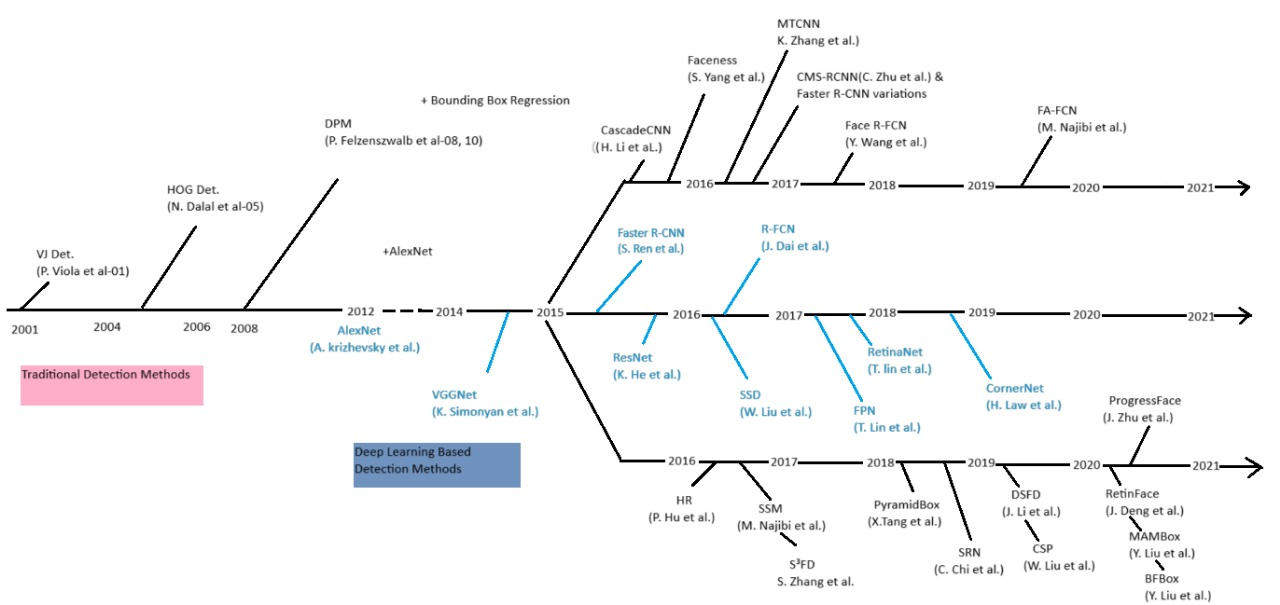
\includegraphics[width=\columnwidth]{components/images/od-timeline.jpg}}
\caption{Object Detection and Face Detection Timeline Overview}
\label{od-timeline}
\end{figure}

Several methods and frameworks, like Viola-Jones \cite{sumanto_viola-jones_2022}, \cite{rani_face_2022}, HOG \cite{rani_face_2022}, MTCNN \cite{rani_face_2022}, MobileNet-SSD \cite{chan_face_2022}, and YOLO-Face \cite{wang_yolov5s-face_2022}, have been utilized to ensure consistent face detection in varying conditions. Once the face is extracted, recognition involves comparing faces within a certain range or threshold, with techniques like PCA and ICA used for accuracy. Lightweight model advancements, such as those based on lightweight models like GhostNet \cite{alansari_ghostfacenets_2023}, have also been explored to meet computational demands for lower end devices.

Authors in \cite{sumanto_viola-jones_2022} used ViolaJones method's on WIDER FACES dataset and achieved a 100\% success rate on detection in groups and meetings, while the previous approaches only managed the highest accuracy results were obtained at 90.9\% for facial images and 75.5\% for non-face images. While these approaches are good under controlled environments their accuracy decreases in uncontrolled environments. Exploring the challenges of detecting faces in uncontrolled environments with varying poses, addressing shortcomings caused by environmental factors, lighting conditions, and image quality authors in \cite{mahesh_smart_2022} proposed an 8-layer Alexnet Convolutional Neural Network (ACNN). By comparing ACNN with the Support Vector Machine (SVM), the research demonstrates that ACNN outperforms SVM, achieving a remarkable 96\% accuracy compared to SVM's 89\% in recognizing faces with varying poses.

Multitask-Net model proposed in \cite{viet_simultaneous_2021} overcomes the challenges of face detection and head pose estimation in digital images which is vital for applications like surveillance. The authors enhances head pose estimation accuracy by leveraging features from face detection and predicts head position and direction simultaneously, utilizing Rotation matrix vectors for face orientation representation to overcome limitations. The results showcase the model's high accuracy, comparable to state-of-the-art methods.

Addressing the issues of missed and false face detection Yongwang Wand et al. \cite{wang_yolov5s-face_2022} proposed a new model based on YOLOV5s by modifying the anchor box size using K-means clustering, embedding an SE attention module on the backbone of YOLOV5s and adding four-scale feature detection for small target faces. This new model gained 3.9\% in mAP and 4.0\% in Recall compared to YOLOV5s. In another paper by Aifian Adi Sufian et al. \cite{chan_face_2022} introduces a two-step face detection framework designed to reduce over-detection in face images and misdetection in non-face images. The method combines feature detection using SSD MobileNet V2 and a geometrical algorithm. When compared to leading algorithms the approach achieved a 91.5\% prediction accuracy. Although it didn't surpass MTCNN and Dlib in accuracy, it was superior in minimizing both over-detection and misdetection.

Farooq et al. \cite{farooq_hybrid_2021} highlights the challenges posed by variations in age, lighting, expressions, and image quality, especially for individuals with dark skin, where existing algorithms tend to perform poorly. To address this racial disparity in facial recognition technology, the authors presents a hybrid algorithm combining Gaussian Model and Explicit Rule Algorithm for skin detection. This innovative approach significantly improves the face detection accuracy for dark-skinned individuals by an impressive 89\%. This underscores the importance of diverse training datasets.

Night time video surveillance arising from varying environmental light conditions can lead to underexposed distant objects and overexposed nearby objects. To combat these issues, the authors in \cite{lu_fusion_2022} introduces the concept of a multi-intensity IR illuminator with periodically varying intensity. The MI3 database is established to assess object detectors in different scenes and illuminations. It evaluates human and face detectors, presenting satisfactory results for simple scenes and proposing a baseline approach for fusion among different illumination intensities.

Khalid M et al. \cite{hosny_privacy_2022} addresses the pressing need for privacy protection in surveillance videos, given the ubiquity of surveillance cameras in our lives. It focuses on safeguarding sensitive regions, particularly people's faces, within surveillance footage. The proposed method employs an object detector, YOLOv3 \cite{aziz_exploring_2020}, to identify the regions and subsequently applies a fast block scrambling technique for obfuscation. Encryption is then applied using secret keys generated from a chaotic logistic map. Notably, the method extends protection to the edges of detected regions to prevent sensitive information leakage. This approach offers practical and robust privacy protection for surveillance videos, ensuring the confidentiality of sensitive data and resilience against potential attacks.

While convolutional neural networks (CNNs) or other Deep learning based approaches have shown promise in face detection, their computational demands can be prohibitive, especially for CPU-based systems as it also adds to the computational complexity and thus requires good hardware which is often not the case with real time surveillance systems, the critical need for lightweight and efficient face detection methods without compromising accuracy was addressed by Muhamad Dwisnanto Putro et al \cite{putro_high_2021}. The authors introduces an optimized architecture, featuring a lightweight CNN with two key modules: a feature extraction backbone and a multilevel detector for accommodating scale variations in face detection. This innovative approach achieves state-of-the-art performance among CPU-based real-time detectors, running at an impressive 53 frames per second (FPS), while requiring fewer than one million parameters.

\section{Face Tracking} \label{section:ft}
A face tracker is a computer vision system or algorithm designed to locate and follow a face in a sequence of frames or a video stream. The primary goal of face tracking is to maintain the identity of a face over time, regardless of facial movements, rotations, occlusions, or changes in facial expressions. Several technologies and algorithms, ranging from classical computer vision techniques to deep learning models, can be used in face tracking. A comprehensive survey of Siamese trackers in visual object tracking (a parent field of face tracking) was done by Milan Ondrasovic et al \cite{ondrasovic_siamese_2021}. Siamese trackers leverage deep learning and similarity learning for tracking objects in videos. They tackle challenges like scale and lighting variations, occlusion, and background clutter. According to authors recent trends involve using deeper backbones like ResNet \cite{aziz_exploring_2020}, multi-level feature fusion, and template updating strategies for improved performance. Cross-correlation with attention mechanisms has shown promise in achieving a balance between speed and accuracy.

Kim et al. \cite{kim_facial_2023} while developing a real time face recognition system used deepSORT as the tracking module. SORT (Simple Online and Realtime Tracking) is to provide a computationally efficient and straightforward method for tracking objects, especially in real-time scenarios. While SORT is computationally efficient and suitable for real-time scenarios, it's primarily designed for scenarios where the number of objects remains relatively constant, and there are minimal interactions or occlusions among objects. For more complex scenarios with numerous occlusions, interactions, and variable object counts, more sophisticated algorithms like DeepSORT (which augments SORT with deep learning-based features).

Multi-face tracking in unconstrained videos to identify and maintain the identities of multiple faces over time is important in real time face recognition system. An online multi-face tracking method was proposed in \cite{weng_online_2023} introduces a two-stage structure: detection alignment and detection association. It aligns face detections with body detections and matches these aligned detections with face or body features to form tracking trajectories. Experiments on benchmark databases demonstrate that utilizing both face and body information significantly enhances tracking performance compared to using only face data, making it competitive with or superior to other online tracking methods for multi-face tracking. Another approach introduces a cross-camera multi-face tracking system for video surveillance \cite{ren_cross-camera_2021}. It combines the Chinese Whisper face clustering algorithm and Double Triplet Networks (DTN) to accurately track pedestrians' faces across different cameras. Experimental results demonstrate its effectiveness, achieving a recognition accuracy of 99.51\% with the DTN MSML Batch OHNM Subspace FOCAL LOSS model. It addresses challenges like small target tracking and occlusion, offering a robust solution for efficient face tracking in surveillance scenarios.

Face tracking in crowded scenes presents a myriad of challenges, central to which is the issue of occlusions where faces are frequently obscured by other individuals or objects. Such environments often result in overlapping faces, making distinct identification and continuous tracking a daunting task. Authors in \cite{barquero_rank-based_2021} focused on enhancing video surveillance systems in crowded and unconstrained scenarios and introduces a novel tracklet reconnection strategy, utilizing rank-based face verification, to extend track lengths by up to 50\% compared to deep learning trackers. This constraint method also reduces identity mixing errors and improves completion rates.

The issues of video face clustering in the context of increasing facial appearance diversity was addressed by Vivek sharma et al. \cite{sharma_video_2020}. They introduced unsupervised methods for feature refinement using deep pre-trained face networks and self-supervised Siamese networks. Discriminative models like Track-supervised Siamese Network (TSiam) and Self-supervised Siamese Network (SSiam) are proposed alongside Variational Autoencoders (VAEs) as a strong generative model baseline. The methods are evaluated on challenging video face clustering datasets and outperform existing state-of-the-art techniques. According to authors the models are computationally efficient, making them suitable for diverse appearance datasets.

\section{Face Recognition} \label{section:fr}
Facial recognition systems generally follow a three-step approach: face detection \ref{section:fd}, face tracking \ref{section:ft}, feature extraction, and identification or verification. While deep learning techniques have significantly improved facial recognition performance, achieving accuracy rates over 99\% on certain datasets, there are concerns about their real-world applicability, especially when recognizing individuals intent on avoiding detection \cite{kim_surveillance_2023}.

Face recognition starts with extracting the face area and its features, which can be a classification challenge to determine if the detected section is a face.

Facial recognition in videos can present ethical dilemmas, particularly in mistakenly identifying innocent bystanders. Most surveillance cameras record at 15 FPS due to storage constraints, but can capture at faster rates. Videos, which provide higher-dimensional data than static images, often give fragmented insights.

Authors in \cite{zhu_webface260m_2023} presents WebFace260M benchmark dataset, WebFace42M benchmark dataset and the Face Recognition Under Inference Time conStraint (FRUITS) protocol for comprehensive evaluation and addresses biased face recognition deployments, including masked and unbiased scenarios. 

Kim et al. \cite{kim_facial_2023} proposed a real-time Criminal Recognition system with 2 major update one is down sampling the input image for reducing the latency during the face detection, whereas high identification accuracy is maintained during the identification step by cropping the face regions from the original high-resolution images. Other update was introduction of Score Dictionary Identification where scores related to the identification results are accumulated for the face ID of each tracked face by creating a dictionary with the tracking ID as a key. The dictionary monitors the score such that when the score exceeds an arbitrary threshold, the system notifies parties of the identification result and transmits the appearance of the criminal.

\subsection{For Devices with limited Computational Power}

Alansari et al. \cite{alansari_ghostfacenets_2023} proposed a deep learning biometric models suitable for devices with limited memory and computational power by the introduction of Ghost modules marks a significant advancement. The model was named GhostFaceNets, lightweight face recognition models, are built upon GhostNetV1 and GhostNetV2, both rooted in Ghost modules. GhostFaceNets, when trained using the ArcFace loss on the refined MS-Celeb-1M dataset, showcased leading performance across benchmarks. They significantly boost efficiency in face verification compared to earlier top mobile CNNs. GhostFaceNets greatly improve efficiency for face verification tasks compared to previous SOTA mobile CNNs, making them suitable for deployment on devices with constrained memory and computational resources. In another such paper \cite{abuzneid_enhanced_2018} authors used back-propagation neural network (BPNN) and correlation-based feature extraction to improve face recognition accuracy. The proposed method achieves higher accuracy with reduced computational cost by generating a new set called the T-Dataset and using a local binary pattern histogram descriptor.

\subsection{Homogeneous Face Recognition}

Homogeneous Face Recognition generally refers to scenarios where the recognition system is designed to handle specific variations or challenges, such as age, pose, lighting, or expression.

With the advent of Covid-19 pandemic a new challenge for face recognition arise which was Masked Face Recognition. Given the global health circumstances since 2020 and the widespread adoption of face masks, masked face recognition has become a notable subfield within Homogeneous Face Recognition, addressing the unique challenges introduced by facial coverings.A masked face recognition algorithm with the combination of Convolutional Neural Network (CNN) and Support Vector Machine (SVM) was proposed by authors in \cite{9914874} where CNN is implemented to train the model, while SVM is used as a label classification method. Two benchmarked datasets, the Real World Masked Face Dataset (RMFD) and the Labelled Face in The Wild Simulated Masked Face Dataset (LFW-SMFD), are used in the experiments. The proposed method achieves a 98.39 percent true acceptance rate on RMFD and 94.29 percent on LFW-SMFD, demonstrating its practicality in recognizing unconstrained face images. Pedro Neto et al. \cite{pedro_neto_beyond_2022} accessed the performance of MFR algorithms was assessed on both masked and occluded face datasets. This assessment was again repeated using a top-performing occluded face recognition algorithm. Finally, to understand the broader context, the evaluation was again performed using algorithms intended for general face recognition. The authors evaluate several approaches for handling masks, including unmasking the input image, unmasking the template generated by a face recognition model, and using a model that is robust to masks.

Age significantly impacts face recognition due to the natural morphological changes that occur over time. Age-related factors can introduce intra-class variations that may pose challenges to recognition algorithms. Age-Invariant Model (AIM) \cite{zhao_towards_2022} was proposed for face recognition in the wild. The model performs cross-age face synthesis and recognition jointly. The AIM model achieves continuous face rejuvenation/aging with photorealistic and identity-preserving properties, without the need for paired data or the true age of testing samples.

\subsection{Heterogeneous Face Recognition}

One other field of face recognition is Heterogeneous Face Recognition (HFR) which refers to the task of matching faces across different domains or modalities. It involves matching a near-infrared (NIR) facial image with a visible light facial image, a sketch of a face with a photographic image, or a thermal image of a face with a regular visible spectrum image etc. A Dual variational generation (DVG-Face) \cite{fu_dvg-face_2022} framework to tackle the heterogeneous face recognition (HFR) problem. It formulates HFR as a dual generation problem and designs a dual variational generator to learn the joint distribution of paired heterogeneous images. A pairwise identity preserving loss is imposed on the generated paired heterogeneous images to ensure their identity consistency. The generated paired heterogeneous images are used to train the HFR network via a contrastive learning mechanism, which yields both domain-invariant and discriminative embedding features. DVG-Face outperforms state-of-the-art methods on seven challenging databases belonging to five HFR tasks, including NIR-VIS, Sketch-Photo, Profile-Frontal Photo, Thermal-VIS, and ID-Camera.
Decheng Liu et al. \cite{liu_heterogeneous_2022} proposed approach with three components, a Graph Convolutional Autoencoder (GCA) for encoding 3D faces into latent representations, a Generative Adversarial Network (GAN) for translating the latent representations of expressive faces into those of neutral faces, and an identity recognition sub-network that utilizes the neutralized latent representations for 3D face recognition. This has practical implications in the field of 3D face recognition and expression neutralization. It offers a method to generate realistic 3D faces with neutral expressions while predicting their identities.
Face Synthesis with Identity-Attribute Disentanglement (FSIAD) \cite{yang_heterogeneous_2022} for Heterogeneous Face Recognition involves two main steps: identity-attribute disentanglement (IAD) and face synthesis module (FSM). Face images are separated into identity-related representations and identity-unrelated representations (attributes) to decrease the correlation between identities and attributes in the IAD step and the FSM is then used to generate a large number of images with stochastic combinations of disentangled identities and attributes, enriching the attribute diversity of synthetic images.

\section{Datasets} \label{section:datasets}

Datasets play a crucial role in the development, training, and evaluation of face detection and recognition systems. They provide researchers with rich resources such as transfer learning where large face datasets can be used to pre-train models, which can then be fine-tuned on smaller, task-specific datasets is often results in better performance than training on the smaller dataset alone.

Requirements of a good dataset are as follows:

\begin{enumerate}
    \item \textbf{Diversity}: The dataset should encompass a wide variety of facial features, expressions, angles, and occlusions. This ensures that the trained models generalize well to real-world scenarios.

    \item \textbf{High Quality Images}: Images should be of high resolution and clarity. Blurry or low-quality images can hinder the performance of detection or recognition systems.

    \item \textbf{Varied Lighting Conditions}: It should include faces under different lighting conditions - from well-lit to poorly lit scenarios - to challenge and enhance the robustness of algorithms.

    \item \textbf{Age Variability}: Faces from different age groups, ranging from infants to the elderly, should be represented to ensure age-invariance in recognition.

    \item \textbf{Demographic Diversity}: A balanced representation of various ethnicities, genders, and backgrounds is essential to prevent biases in the resulting models.

    \item \textbf{Annotations}: Precise annotations, including bounding boxes for detection and identity labels for recognition, are crucial.

    \item \textbf{Temporal Data}: For video-based recognition systems, the dataset should include video sequences to account for temporal variations and movements.

    \item \textbf{Real-world Scenarios}: Inclusion of "in-the-wild" images or videos where faces are naturally occluded, or in varied expressions and postures, simulates real-world challenges.

    \item \textbf{Scalability}: A good dataset should be large enough to train deep learning models, which often require vast amounts of data.

    \item \textbf{Consent and Ethics}: All data should be collected with proper consent, ensuring the privacy and rights of the individuals are respected.
\end{enumerate}



WebFace260M benchmark \cite{zhu_webface260m_2023}, an ultra-large-scale dataset comprising 4 million identities and 260 million faces was introduced to bridge the data gap between academia and industry. The dataset was still refined by employing the Cleaning Automatically by Self-Training (CAST) pipeline,into WebFace42M, with 2 million identities and 42 million faces. The benchmark and cleaned dataset facilitate efficient model training, resulting in improved face recognition performance and potential solutions for bias mitigation and privacy concerns in the field. The benchmark and cleaned dataset facilitate efficient model training, resulting in improved face recognition performance and potential solutions for bias mitigation and privacy concerns in the field.

Zhongyuan Wang et al. \cite{wang_masked_2023} proposes three types of masked face datasets: Masked Face Detection Dataset (MFDD), Real-world Masked Face Recognition Dataset (RMFRD), and Simulated Masked Face Recognition Dataset (SMFRD). The Real-world Masked Face Recognition Dataset (RMFRD) is claimed to be the world's largest real-world masked face dataset by the authors. Although the details of the specific methods used in developing the datasets are not mentioned in the provided sources. DVG-Face framework \cite{fu_dvg-face_2022} was evaluated on seven challenging databases belonging to five HFR tasks, including NIR-VIS, Sketch-Photo, Profile-Frontal Photo, Thermal-VIS, and ID-Camera, and achieves superior performances over state-of-the-art methods and outperforms them. Zhao et al. \cite{zhao_towards_2022} curated a new large-scale Cross-Age Face Recognition (CAFR) benchmark dataset to facilitate research in age-invariant face recognition for their AIM model. Extensive experiments are conducted on the CAFR dataset and other cross-age datasets (MORPH, CACD, FG-NET) to demonstrate the superiority of the proposed AIM model over existing techniques. The AIM model is further benchmarked on unconstrained face recognition datasets (YTF, IJB-C) to verify its generalization ability in recognizing faces in the wild.

Authors in \cite{abuzneid_enhanced_2018} used 3 datasets YALE and AT\&T for testing the proposed framework and evaluated their method on the LFW dataset, which is a state-of-the-art benchmark dataset for face recognition.

Detection in a controlled environment often leads to good results but when the model is deployed in an uncontrolled environment with noise, occlusion, extrnal lighting, makeups etc often referred as ``in the wild" then the accuracy drops. But there are dataset with these kinds of images. One such dataset is the WIDER FACE dataset, which is used as a training dataset for the CNN based lightweight detector in \cite{putro_high_2021}. It contains 32,203 images, with 12,800 images specifically used for training the detector. Augmentation techniques are applied to enrich the training data and prevent overfitting during the training process. The second dataset is the PASCAL face dataset \cite{putro_high_2021}, which consists of 851 images with 1335 labelled faces. This dataset is a subset of the PASCAL VOC dataset and includes variations in pose and background, both indoor and outdoor.

Datasets like VGGFace2 and MS-Celeb-1M, which primarily contain data from young, facially beautiful celebrities with makeup, are biased in terms of age and facial appearance, leading to potential performance issues when using pretrained models from these datasets on different audiences \cite{wanyonyi_open-source_2022}.

Tables \ref{det-ds} and \ref{rec-ds} contains a list of popular publicly available datasets found in the literature survey:

\begin{table}[htbp]
\caption{Detection Datasets}
\begin{center}
\begin{tabularx}{\columnwidth}{|X|c|X|}
\hline
\textbf{Dataset} & \textbf{Year}& \textbf{Size} \\
\hline
VGGFace2 \cite{kim_face_2022} & 2018 & 3.31 million images of 9,131 subjects \\
\hline
WIDER Face \cite{kim_face_2022} & 2016 & 32,203 images with 393,703 annotated face bounding boxes \\
\hline
VGGFace2 \cite{kim_face_2022} & 2018 & 3.31 million images of 9,131 subjects \\
\hline
PASCAL Face \cite{feng_detect_2022} & 2012 & 1,335 faces from 851 images \\
\hline
\end{tabularx}
\label{det-ds}
\end{center}
\end{table}
    
    
\begin{table}[htbp]
\caption{Recognition Datasets}
\begin{center}
\begin{tabularx}{\columnwidth}{|X|c|X|}
\hline
\textbf{Dataset} & \textbf{Year}& \textbf{Size} \\
\hline
MS-Celeb-1M \cite{wanyonyi_open-source_2022} & 2016 & 10 million images of 100,000 celebrities \\
\hline
LFW \cite{kim_face_2022} & 2007 & 13,000 images of 5,749 distinct individuals \\
\hline
CASIA NIR-VIS 2.0 \cite{liu_heterogeneous_2022} & 2007 & 17,580 images from 725 subjects \\
\hline
ChokePoint \cite{barquero_rank-based_2021} & 2011 & 54 video sequences captured from 6 different camera views \\
\hline
\end{tabularx}
\label{rec-ds}
\end{center}
\end{table}

\section{Proposed System}
The core of the proposed system is a real-time face recognition engine that encompasses multiple components: face detection, face tracking, face encoding, and identification. The system will leverage state-of-the-art algorithms, deep learning methodologies, and vast datasets to ensure optimal accuracy and speed, even in challenging scenarios encountered by law enforcement agencies. This engine integrates seamlessly with a database of known individuals and offers a user-friendly interface for law enforcement personnel. At its core, the system is engineered to overcome the challenges inherent in the real time face recognition scenarios, including occlusion handling, dynamic background, crowded scenarios etc. This proposed system consists of a set of cutting-edge components and features that collectively redefine the real time face recognition:

	\subsection{Face Detection Module}
		The face detection module prioritizes real-time processing and emphasizes rotation invariance and region-of-interest determination. The primary task is to have capability to process live video feeds instantly. As it's a real time video stream so the latency should be pretty low and the detection accuracy should be high. This is the heart of the entire architecture as without detection there is no point of recognition so the detection module should be fast and accurate to identify the faces in the wild where there are challenges like occlusion, dynamic background and heavy crowd etc. The module in order to ace encompasses deep learning-based algorithms like RetinaFace, YOLO or SSD for rapid and accurate detection of faces in images or video streams as they are the current state of the art algorithms. It prioritizes regions in a frame with higher chances of containing faces, optimizing computational resources. It also incorporates multi-scale detection to capture faces of varying sizes and at different distances from the camera.
		The face detection module employs advanced algorithms to detect faces in the wild.
		

	\subsection{Face Tracking Module}
		As faces are detected, they are tracked over time using a sophisticated module that ensures temporal consistency, can simultaneously track multiple faces in crowded scenarios, and employs predictive pathing to anticipate movements. For this advanced tracking algorithms such as deepSORT or Siamese networks are employed. They are designed to maintain continuous tracking, even when the subject moves, turns their face, or gets partially obscured. The main task is to predicts and anticipates the path a face might take, ensuring smoother tracking.

	\subsection{Face Encoding and Identification Module}
		Once tracked, faces undergo deep feature extraction within the identification module that matches them rapidly against a vast database while employing anti-spoofing techniques. This module extracts facial features and converts them into a compact vector (or embedding) using neural networks like ResNet or VGG. Then it compares the derived embeddings with a database of known embeddings to ascertain identity. As there would always be some faces that will be probable the module integrates a threshold mechanism to eliminate false positives and ensure high-confidence identifications. Once the module is confident enough an alert will be generated and given to the respective authorities about the detection.

	\subsection{Database Integration}
		The system seamlessly integrates with an encrypted, secure, and fast-access database storing facial embeddings of known individuals. This way they incorporates a periodic update mechanism to add new embeddings and ensure the database remains current. It would incorporate a tagging mechanism to efficiently tag and categorize faces for quicker searches. Regular backups should also be taken to prevent data loss and facilitate recovery. The system's database structure prioritizes differential updates, ensuring minimal lag.

	\subsection{Training and Update Mechanism}
		The proposed system suggests instead of complete retraining, the training should be incremental and the thus updates the model with new data increments only. The model evaluation should also be automated and continuous evaluation of model performance and automatic rollback should be done if a newer version performs poorly. It also Incorporate feedback from users to refine and improve models.

	\subsection{Performance Analytics}
		The reports should be customizable to suit specific requirements and real-time alerts should be given for any anomalies or performance drops. The module provides trends and historical data for long-term performance assessment.
		
	\subsection{Cross-Platform Accessibility}
		The proposed system is designed with accessibility in mind. It is accessible across various platforms, including web browsers, mobile applications, and other embedded devices. This cross-platform approach ensures that users can engage with the system on their preferred devices, making it versatile and user-friendly.
	\chapter{REQUIREMENT ANALYSIS}

% \section{Introduction}
% 	This project aims to empower users to make informed fashion choices and enhance their online shopping experience by seamlessly integrating AI algorithms for clothing recommendations and virtual try-on technology. In an era where online shopping dominates, our system seeks to empower consumers with a personalized shopping experience.

% 	\subsection{Purpose}
% 		The main goals of this project are to elevate the online shopping experience of customers by using AI to provide them with personalized clothing recommendations and AR virtual try-on, to reduce uncertainty associated with online purchases and by extension, reduce item return rates.

% 	\subsection{Project Scope}
% 		The project has the following scope:

% 		\begin{enumerate}
% 			\item \textbf{Fashion embedding:} Fashion embedding is a pivotal component, serving as the foundation for further tasks.
% 				\begin{enumerate}
% 					\item \textit{High-dimensional representation:} The project will transform clothing items into high-dimensional representations in a latent space. Each item will be associated with a vector that encodes its unique features and attributes.
% 					\item \textit{Recommendation:} These fashion embeddings will play a fundamental role in the recommendation system. They will enable the model to identify similarities and compatibilities between items, effectively suggesting products based on user preferences and past interactions. Recommendations will be made by locating items with embeddings closely aligned with the user's preferences.
% 					\item \textit{Retrieval:} The fashion embeddings will facilitate efficient and accurate retrieval of items. Users will be able to search for specific items or styles by querying the embedded space, and the system will quickly locate relevant matches.
% 					\item \textit{Semantic understanding:} The high-dimensional embeddings will capture the semantic meaning and context of fashion items, going beyond visual features. This means that items with similar semantic attributes can be effectively grouped together.
% 				\end{enumerate}
% 			\item \textbf{Feature extractor:} Use deep learning to train a feature extractor which can segment parts of the upper body to provide user features for attribute-based recommendations, and to detect rendering regions for virtual try-on.
% 			\item \textbf{AI-based recommender:} Design and deploy a recommendation system that utilizes collaborative and content-based filtering to generate personalized clothing recommendations.
% 				\begin{enumerate}
% 					\item \textit{Train with body dimensions:} Fine-tune system to take into account various body dimensions, such as waist size, chest measurements, and height.
% 					\item \textit{Recommendations tailored to physique:} Provide clothing recommendations suitable for lean to average body sizes of average body length. Offer suggestions that are not only stylish but also appropriately sized.
% 				\end{enumerate}
% 			\item \textbf{AR virtual try-on:} Develop an AR-based virtual try-on system that allows users to visualize and interact with clothing items in real-time.
% 				\begin{enumerate}
% 					\item \textit{Dynamic and responsive:} Design a dynamic and responsive system with which users can try on multiple clothing items and evaluate them one by one.
% 					\item \textit{Device compatibility:} Ensure system is compatible with a range of devices, including smartphones, tablets, and desktops, making it accessible to a wide user base.
% 					\item \textit{User-Friendly Interface:} Design an user interface which is intuitive and user-friendly, ensuring that users can easily navigate and interact with the virtual try-on features.
% 				\end{enumerate}
% 		\end{enumerate}

% \section{Overall Description}
% 	\subsection{Product Perspective}
% 		Our project operates within the context of the broader e-commerce and fashion retail landscape. It aims to integrate with e-commerce platforms, acting as an enhancement to the shopping experience. This system augments traditional online shopping by providing intelligent clothing recommendations and a virtual try-on feature. It does not replace or compete with e-commerce platforms but complements their functionality, aiming to boost user engagement and sales. By focusing on user experience, the project seeks to align with the goals of e-commerce businesses, creating a symbiotic relationship that benefits both consumers and retailers.
	
% 	\subsection{Product Functions}
% 		The project has the following product functions:

% 		\begin{enumerate}
% 			\item \textbf{User profiles:} Users can create accounts and profiles, providing personal information, style preferences, and body measurements. Profiles are used to tailor clothing recommendations to individual user preferences.
% 			\item \textbf{Clothing recommender:} Utilizes AI algorithms to analyze user data and style preferences and generates personalized clothing recommendations based on the user's profile.
% 			\item \textbf{Search and browsing:} Allows users to search for clothing items or browse through a selection of recommended items. Filters, sorting options, and search functionality enhance the browsing experience.
% 			\item \textbf{Virtual try-On:} Employs augmented reality (AR) technology to enable users to virtually try on clothing items. Overlays selected garments on the user's real-time image or avatar to visualize fit and appearance. Supports various angles and poses to ensure an accurate representation.
% 			\item \textbf{User feedback:} Allows users to rate and review purchased items. Collects valuable feedback to improve the recommendation system.
% 		\end{enumerate}

% 		\begin{figure}
% 			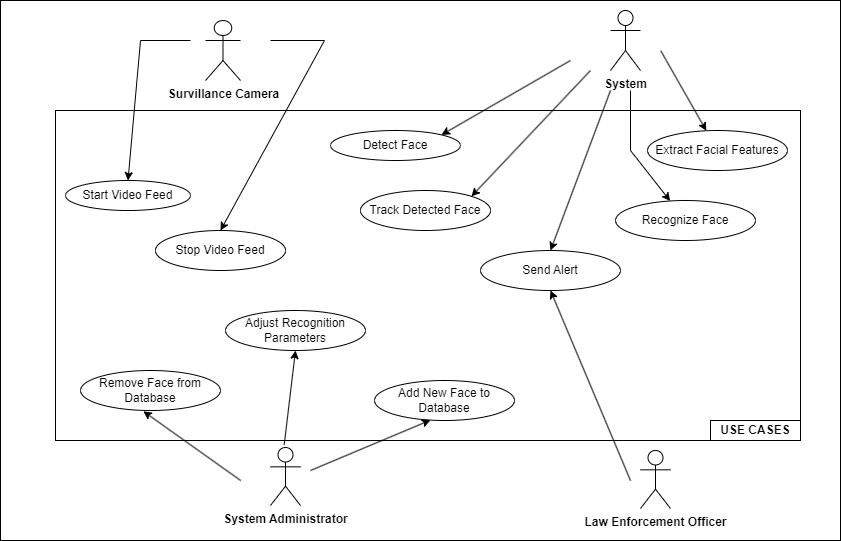
\includegraphics[width=\textwidth]{components/images/use-case.png}
% 			\caption{Use-case diagram}
% 			\label{fig:use-case}
% 		\end{figure}

% 	\subsection{User Classes and Characteristics}
% 		The project has the following user classes: 

% 		\begin{enumerate}
% 			\item \textbf{Online shoppers:}
% 				\begin{itemize}
% 					\item \textit{Characteristics:} Shoppers are the primary end-users of the system. They have varying fashion preferences and seek clothing recommendations that align with their personal style and body type. Shoppers may have different levels of technological proficiency, from tech-savvy individuals to those with limited technology experience.
% 					\item \textit{Usage:} Shoppers use the system to search for clothing items, receive personalized recommendations, and virtually try on garments. They provide feedback and ratings to refine future recommendations.
% 				\end{itemize}
% 			\item \textbf{Retailers and fashion brands:}
% 				\begin{itemize}
% 					\item \textit{Characteristics:} Retailers and fashion brands represent business partners or clients who wish to integrate the recommendation and virtual try-on system into their e-commerce platforms. They possess in-depth knowledge of their product catalogs and seek to improve customer engagement and sales.
% 					\item \textit{Usage:} Retailers and fashion brands collaborate with the development team to integrate the system into their online stores. They may provide fashion catalogs, branding assets, and participate in system customization.
% 				\end{itemize}
% 			\item \textbf{Fashion designers and stylists:}
% 				\begin{itemize}
% 					\item \textit{Characteristics:} Fashion designers and stylists may collaborate with the system to showcase their clothing collections or styling expertise. They are experts in fashion trends, design, and styling.
% 					\item \textit{Usage:} Designers and stylists work with retailers to curate clothing collections and styles for the system. They may also provide fashion tips, styling advice, or content to enrich the user experience.
% 				\end{itemize}
% 			\item \textbf{Data analysts and AI specialists:}
% 				\begin{itemize}
% 					\item \textit{Characteristics:} Data analysts and AI specialists are responsible for fine-tuning the recommendation algorithms and ensuring the system's AI components work optimally. They possess expertise in data analysis and machine learning.
% 					\item \textit{Usage:} Data analysts and AI specialists continuously improve recommendation algorithms, analyze user data for patterns, and adapt the system to evolving fashion trends and customer preferences.
% 				\end{itemize}
% 		\end{enumerate}

% \section{Specific Requirements}
% 	\subsection{Operating Environment}
% 		The operating environment of our project is as follows:

% 		\begin{enumerate}
% 			\item \textbf{Software requirements:}
% 				\begin{itemize}
% 					\item \textit{Operating system:} The target end-user operating system may be any of the following platforms which support the ONNX Runtime \cite{onnxruntimeCompatibility}:
% 						\begin{itemize}
% 							\item Windows 10 1709+
% 							\item Linux distributions supported by .NET Core
% 							\item Mac 10.14+ (Mojave)
% 							\item Android 28+ (v9 ``Pie")
% 							\item iOS 12+
% 						\end{itemize}
% 					\item \textit{Web browsers:} It should be accessible through popular web browsers like Google Chrome, Mozilla Firefox, Safari, and Microsoft Edge for web-based interfaces.
% 					\item \textit{AR framework:} A robust AR framework such as AR.js for web-based AR experiences, should be integrated.
% 					\item \textit{Database management:} The project requires a database management system for user profiles, clothing item information, and preference data. Document-based NoSQL options like Apache Cassandra can be considered.
% 					\item \textit{Programming languages and libraries:} Development will involve languages like Python and JavaScript, and frameworks like PyTorch and Huggingface Transformers and Optimum for machine learning tasks.
% 					\item \textit{Machine learning inference:} A cross-platform machine learning runtime like ONNX Runtime which supports the ONNX format, an open standard for machine learning interoperability.
% 					\item \textit{Web development stack:} For web-based interfaces, a stack including HTML, CSS, JavaScript, and backend frameworks like Node.js and Express will be employed.
% 				\end{itemize}
% 			\item \textbf{Hardware requirements:}
% 			\begin{itemize}
% 				\item \textit{User devices:} The project is intended to work on a range of user devices like smartphones, tablets, laptops, and desktop computers.
% 				\item \textit{Cameras and sensors:} Devices should have integrated or attachable cameras and sensors capable of capturing user images and surroundings for the virtual try-on feature.
% 				\item \textit{CPU:} Any modern multi-core processor with a clock speed of at least 2.5 GHz.
% 				\item \textit{GPU:}
% 					\begin{itemize}
% 						\item Training requirement: A video-card with minimum 8GB VRAM for deep learning tasks.
% 						\item End-user inference requirement: Any GPU which supports Vulkan APIs.
% 					\end{itemize}
% 				\item \textit{Internet connectivity:} A stable internet connection is essential for real-time communication with the server, image processing, and rendering of AR elements.
% 			\end{itemize}
% 		\end{enumerate}
	
% 	\subsection{Design Philosophies}
% 		\begin{enumerate}
% 			\item \textbf{User-centric design:} Our design philosophy places the user at the center of the system. We prioritize creating an intuitive and seamless user experience that accommodates users of various demographics and technological backgrounds. User feedback will continuously inform design improvements.
% 			\item \textbf{Personalization:} The system will employ machine learning algorithms to create a highly personalized experience. User preferences and feedback will be used to tailor clothing recommendations and enhance the virtual try-on experience.
% 			\item \textbf{Scalability:} The design will be modular and scalable to accommodate a growing user base and evolving technological trends. This approach allows for easy integration of new features and accommodates increased usage loads.
% 			\item \textbf{Security and privacy:} Security and privacy will be fundamental to the design, with strong encryption protocols for data protection. Users' personal information and imagery will be handled with the utmost care, and adherence to data protection regulations is a priority.
% 		\end{enumerate}

% 	\subsection{Implementation Philosophies}
% 		\begin{enumerate}
% 			\item \textbf{State-of-the-Art AI:} Implementation will involve integrating state-of-the-art machine learning and computer vision techniques to ensure accurate clothing recommendations and realistic virtual try-on experiences. We will employ libraries and frameworks with active development and community support.
% 			\item \textbf{Cross-platform compatibility:} The system will be developed with cross platform compatibility in mind. Web interfaces will be developed to ensure that users can access and utilize the system seamlessly on various devices.
% 			\item \textbf{Continuous testing and iteration:} Agile development methodologies will be used to enable continuous testing, feedback, and iteration. This approach allows us to respond to user needs, refine algorithms, and enhance system performance throughout development.
% 		\end{enumerate}

% 	\subsection{Constraints}
% 		\begin{enumerate}
% 			\item \textbf{Data Privacy and Compliance:} The project must adhere to strict data privacy regulations. This imposes constraints on how user data is collected, stored, and utilized.
% 			\item \textbf{Resource Limitations:} The project will operate within resource constraints, including budget and available hardware resources, which may affect the system's scalability and performance.
% 			\item \textbf{Technological Compatibility:} The system must work across a wide range of devices and platforms, which presents constraints related to compatibility and performance optimization.
% 			\item \textbf{User Connectivity:} User experience may be affected by the quality of the user's internet connection, especially when utilizing the augmented reality feature. Ensuring a functional experience even in low-bandwidth situations is a constraint.
% 		\end{enumerate}

% \section{External Interface Requirements}
% 	\subsection{User Interfaces}
% 		The primary user interface will be web-based and accessible via standard web browsers. It should be compatible with popular web browsers, including but not limited to Google Chrome, Mozilla Firefox, Microsoft Edge, and Safari. The user interface should be responsive, adapting to various screen sizes, including desktops, tablets, and mobile devices.

% 		The virtual try-on interface relies on AR and should be compatible with most devices. It must support features such as real-time clothing overlay and interactive controls for users to try on clothing items seamlessly.
	
% 	\subsection{Hardware Interfaces}
% 		The virtual try-on feature requires the use of cameras and sensors. Our system should interface with these devices to capture images and detect user movements for an immersive AR experience. These interfaces should be compatible with a range of devices.

% 	\subsection{Software Interfaces}
% 		\subsubsection{Clothing Recommendation Interface}
% 			The system will interface with a clothing recommendation algorithm to leverage advanced recommendation algorithms for personalized clothing suggestions.

% 			Requirements:
% 			\begin{enumerate}
% 				\item The system should send user profile and preferences data to the recommendation algorithm.
% 				\item The algorithm should return a list of recommended clothing items.
% 				\item The interface should allow for updates to the recommendation algorithm without affecting core system functionality.
% 			\end{enumerate}
		
% 		\subsubsection{AR Virtual Try-On Interface}
% 			The system will interface with an AR module for virtual clothing try-on to enable users to visualize clothing items on themselves in real-time.

% 			Requirements:
% 			\begin{enumerate}
% 				\item The AR module must support 3D model rendering of clothing items on user images.
% 				\item It should provide accurate real-time visualization.
% 				\item The system should send data about selected clothing items to the AR module for rendering.
% 				\item The AR module should return rendered images or video streams of users with clothing items superimposed.
% 			\end{enumerate}

% 		\subsubsection{User Profile and Preferences Data Interface}
% 			The system will interact with user profile and preferences data to gather information about user preferences and characteristics for clothing recommendations.

% 			Requirements:
% 			\begin{enumerate}
% 				\item The system must allow users to create and update their profiles.
% 				\item It should securely store and retrieve user data.
% 				\item The interface must be compliant with data protection regulations.
% 			\end{enumerate}

% \section{Other Nonfunctional Requirements}
% 	\subsection{Performance Requirements}
% 		The system should be able to read and understand the human body and be able to parse the areas of interests, generate outfit accordingly and finally, render the subject in real-time through augmented reality.
		
% 		\subsubsection{Resource utilization}
% 			For the system to be compatible with majority devices including low powered mobiles and tablets, the resource utilization should be kept to minimum without affecting the quality of output.

% 		\subsubsection{Feedback duration}
% 			As expected of the try-on systems, the system should be able to provide feedback on the subject in real-time. Processing time should be kept as low as possible for better experience for user.

% 		\subsubsection{Feedback quality}
% 			The system should generate personalized outfit and the subject should be able to judge the proposed style and size on itself. The process should be both convenient and rewarding for the user.
		
% 	\subsection{Safety and Security Requirements}
% 		\begin{enumerate}
% 			\item \textbf{Privacy compliance:} The user shouldn't be concerned about disclosure of his/her features to open userbase. The system should only parse the regions of interest for building the metrics of generation and should not intent to perform any malicious operations.
% 			\item \textbf{Ethics:} The system should not delve into inappropriate outfit generation and should take into account of user's modesty. The system shouldn't be biased towards certain age groups, races or color.
% 			\item \textbf{Compliances:} The system should adhere to rules and compliances stated by the authorities and stakeholders and should limit it's working domain to that specified be the compliances.
% 		\end{enumerate}
	
% 	\subsection{Acceptance Criteria}
% 		Give the scenario where the user has selected certain clothes according to their preferences and is expecting the system to generate the outfit on their body so that they can judge the style and the overall look of the outfit, the user lets the camera record their body. Both the subject body features and generated recommendations are input for the system.

% 		When the user selects generate outfit option after selection of styles recommended or chosen by himself/herself. The system segments the features from the subject and tries to wrap the outfit around them. If the system is well trained on personalized recommendation and virtual try-on, the system successfully generates the outfit personalized to the subject and provides the rendered view in augmented reality.

% 	\subsection{Software Quality Attributes}
% 		\begin{enumerate}
% 			\item \textbf{Reliability:} The system should be dependable, providing accurate clothing recommendations and ensuring that the virtual try-on feature functions consistently without errors or crashes.
% 			\item \textbf{Usability:} User interfaces should be intuitive and user-friendly, making it easy for customers to navigate the system and obtain clothing suggestions effortlessly.
% 			\item \textbf{Maintainability:} The codebase should be well-organized, documented, and structured to facilitate updates, enhancements, and bug fixes.
% 			\item \textbf{Flexibility:} The system should adapt to changes in user preferences, allowing for the integration of new fashion items and the modification of recommendation algorithms.
% 			\item \textbf{Robustness:} The system should be able to handle unexpected inputs or situations without crashing or providing inaccurate results.
% 		\end{enumerate}

% \section{Future Scope}
% 	The project opens up the following future developments:

% 	\begin{enumerate}
% 		\item Inclusion of more body types.
% 		\item Extended clothing categories and varieties.
% 		\item Multi-modal integration such as voice-activated commands and gesture-based interactions for enhanced virtual try-ons.
% 		\item Integration of social media elements.
% 		\item Integration with wearable technology.
% 		\item Fashion trend analysis and prediction to aide recommendations.
% 	\end{enumerate}

\section{Introduction}
    In the rapidly advancing domain of law enforcement, the emergence of real-time face recognition is a pivotal tool for enhancing security, optimizing response times, and bolstering crime prevention and investigative capabilities. However, the practical deployment of such real-time facial recognition systems is rife with complexities, especially when applied to the dynamic and often unpredictable scenarios encountered in law enforcement. Challenges such as occlusions, dynamic backgrounds, and the inherent intricacies of tracking multiple individuals in crowded settings underscore the need for robust, efficient, and reliable systems. This section is geared towards detailing the prerequisites, desired functionalities, and specifications for the development of an advanced real-time face recognition system tailored to meet the unique needs and challenges of law enforcement.
    
    \subsection{Purpose}
    Develop a real-time face recognition system tailored specifically for law enforcement. This system is designed to enhance security measures, facilitate faster responses, and offer more effective crime prevention and investigation by swiftly and accurately identifying individuals in the field. It aims to navigate and address the inherent challenges in real-world law enforcement scenarios, such as facial occlusions due to masks or sunglasses, recognition in crowded settings, and varying backgrounds. The system seeks to optimize the process of face detection, tracking, and recognition, ensuring it meets the unique demands and high stakes of law enforcement scenarios.
    
    \subsection{Project Scope}
    This project's scope includes creating an real time face recognition system that can match the detected face with a database in real-time, allowing for swift identification. It also consists of a secure and scalable database to store facial data. This database can be updated as required, allowing for additions, modifications, or deletions.    Providing thorough documentation to help users deploy and utilize the system efficiently is another aspect of the scope. The project's scope is set to ensure that the system is not just accurate but also practical for the high-stakes, dynamic environments in which law enforcement operates.


\section{Overall Description}
    \subsection{Product Perspective}
        It operates within a broader system perspective, integrating seamlessly with existing law enforcement surveillance infrastructure. This system serves as a modular component, capable of functioning both independently and as an integral part of the surveillance ecosystem. Its main functions encompass face detection, tracking, real-time recognition, and alert generation. The face recognition system complements the surveillance network by enhancing security and investigative capabilities, and it offers a vital tool that promises to revolutionize law enforcement operations. Its versatility in either standalone operation or integration into existing systems ensures flexibility and adaptability to various law enforcement scenarios, positioning it as a valuable asset in the realm of real-time face recognition for law enforcement purposes.
    
    \subsection{Product Functions}
        The product, a real-time face recognition system for law enforcement, has several core functions. Some of the functions are:
        \begin{itemize}
            \item \textbf{Face Detection:} The system can scan and identify human faces from various sources such as images, videos, and live surveillance feeds. This function can handle multiple faces simultaneously even in crowded scenes and identify them in varying lighting conditions and angles.
            \item \textbf{Face Tracking:} After detecting faces, the system has the capability to track individual faces across a sequence of frames or video streams. It maintains continuity, even if the face undergoes temporary occlusions, movements, or changes in expression.
            \item \textbf{Real-time Face Recognition:} By comparing detected faces against a database of known individuals, the system can swiftly and accurately identify persons of interest. This function is invaluable in law enforcement settings, where the prompt identification of a suspect or missing person can be crucial.
            \item \textbf{Alert Generation:} When the system identifies a match or encounters a predefined scenario (e.g., an individual from a watchlist appearing in a restricted area), it generates real-time alerts. These notifications can be forwarded to law enforcement officers or other relevant personnel for immediate action.
            \item \textbf{Integration with Existing Surveillance Systems:} The product seamlessly integrates with current surveillance infrastructure, making it a plug-and-play solution that enhances the capabilities of existing systems.
        \end{itemize}
    
    \subsection{User Classes and Characteristics}
        The various user classes interacts with the system differently and has unique needs, which should be considered during the system design and development phase to ensure a comprehensive and efficient product. 
        \begin{enumerate}
            \item \textbf{Law Enforcement Officers (On-field):}
                \begin{itemize}
                    \item Typically operate in the field and require real-time data.
                    \item Need simple, intuitive interfaces due to the critical nature of their work.
                    \item May not have extensive technical expertise but are trained for basic operations.
                    \item Rely heavily on the accuracy and timeliness of the face recognition system.
                    \item Require alerts and notifications for immediate actions.     
                \end{itemize}
            \item \textbf{Surveillance Operators:}
                \begin{itemize}
                    \item Usually stationed in control rooms monitoring multiple feeds.
                    \item Need advanced filtering options to focus on specific camera feeds or regions.
                    \item Have a moderate level of technical expertise.
                    \item Need tools for playback, zoom, and other video controls.
                    \item Prioritize system stability and seamless integration with existing surveillance infrastructure.    
                \end{itemize}
            \item \textbf{Forensics and Investigation Teams:}
                \begin{itemize}
                    \item Use the system for post-incident analysis rather than real-time monitoring.
                    \item Require advanced search functionalities, including partial face recognition, timestamp filtering, and location-based searching.
                    \item Need capabilities for evidence documentation, including exporting clips, snapshots, or recognition reports.
                    \item Highly trained and have a mix of technical and investigative expertise. 
                \end{itemize}
            \item \textbf{System Administrators:}
                \begin{itemize}
                    \item Responsible for the maintenance, updates, and overall health of the face recognition system.
                    \item Need advanced administrative controls, including user management, system diagnostics, and backup utilities.
                    \item Highly technical and have a deep understanding of the system's infrastructure and its integration points.   
                \end{itemize}
            
        \end{enumerate}
    
    \subsection{Operating Environment}
        The system will operate on Windows-based systems primarily. It will require a sufficiently powerful CPU and GPU to run efficiently. Detailed description is provided below:
        \begin{enumerate}
            \item \textbf{Hardware Platform:}
                The software is designed to operate on a variety of hardware platforms, but it performs optimally with the following specifications:
                \begin{itemize}
                    \item \textit{CPU:} A modern multi-core processor (e.g., Intel Core i5 or AMD Ryzen 5) with a clock speed of at least 2.5 GHz.
                    \item \textit{GPU:} Nvidia GeForce or AMD Radeon series GPUs are recommended.
                    \item \textit{RAM:} A minimum of 8 GB of RAM for efficient processing and multitasking.
                    \item \textit{Storage:} Adequate free storage space for the operating system (preferably Solid-State Drive).
                    \item \textit{Surveillance Cameras:} Integration with a wide array of camera models and types, including IP cameras, PTZ cameras, thermal imaging cameras, and body-worn cameras.
                    \item \textit{End-User Devices:} Compatible with standard workstations in control rooms, mobile devices for on-field officers, and specialized terminals for surveillance operators.
                \end{itemize}
            \item \textbf{Software Environment:}
                \begin{itemize}
                    \item \textit{Operating System:} Compatible with Windows 10 and later versions (64-bit).
                    \item \textit{Database Management:} Compatible with leading database management systems, ensuring smooth and efficient storage and retrieval of facial data, recognition logs, and system analytics.
                    \item \textit{Integration Modules:} Built-in connectors for integrating with existing surveillance software, law enforcement databases, and other critical third-party systems.                    
                \end{itemize}
            \item \textbf{Network Environment: }
                \begin{itemize}
                    \item \textit{Local Area Network (LAN):} Designed to operate efficiently within intranet environments, especially for high-bandwidth operations like streaming video feeds.
                    \item \textit{Wide Area Network (WAN):} Capable of remote operations, ideal for connecting distant locations, and enabling mobile access.
                    \item \textit{Internet:} Provides secure internet-based access for remote surveillance monitoring, administrative tasks, and system updates. Uses encrypted connections and complies with best practices for cybersecurity.
                \end{itemize}
        \end{enumerate}
        By ensuring compatibility with these hardware and software components, the system can effectively operate and provide reliable results for its users.
    
    
    \subsection{Design and Implementation Constraints}
        \begin{enumerate}
            \item \textbf{Hardware Limitations}
            The system's efficiency is directly proportional to the hardware it operates on. Advanced facial recognition algorithms, especially those leveraging deep learning, require powerful computational resources. The minimum hardware requirement needs to be strictly adhered to for optimal performance.
            \item \textbf{Data Privacy and Security}
            Given the sensitive nature of facial data, strict encryption and cybersecurity protocols must be maintained. The system must comply with prevailing data protection regulations and laws.
            \item \textbf{Network Dependence}
            The system's efficiency depends on the stability and speed of the network. Any latency or network disruptions can impede its real-time recognition capabilities.
            \item \textbf{Integration with Existing Systems}
            The design must be adaptable and modular to ensure smooth integration with various surveillance systems, databases, and third-party tools already in use by law enforcement agencies.
            \item \textbf{Software Licensing}
            Some third-party tools, libraries, or software components that the system might rely on could have licensing restrictions, which could impact the distribution, modification, or commercialization of the system.
            \item \textbf{Continuous Training}
            For the system to maintain its effectiveness, the underlying models might need periodic retraining, which would require access to fresh, labelled data. This ongoing need can be a constraint for maintaining the system's accuracy over time.
            \item  \textbf{Scalability}
            As the user base grows and more data is fed into the system, its design should allow for easy scalability without a significant overhaul.
        \end{enumerate}
    
    \subsection{User Documentation}
        Comprehensive user documentation will be provided, including installation guides, usage instructions, and troubleshooting tips. Users will also have access to a knowledge base for common issues and solutions. Some documentation that will be provided are:
        \begin{enumerate}
                \item \textbf{User Manual:}
                    \begin{itemize}
                        \item \textit{Delivery Format:} PDF and online knowledge base.
                        \item \textit{Standards:} The user manual will adhere to standard technical writing conventions, including clear instructions, diagrams, and an easy-to-navigate structure.
                    \end{itemize}
                \item \textbf{Video Tutorials:}
                    \begin{itemize}
                        \item \textit{Delivery Format:} Video files (e.g., MP4) hosted on a dedicated platform (e.g., YouTube or GitHub).
                        \item \textit{Standards:} Video tutorials will be created with professional video editing software and include voiceovers or captions for accessibility.    
                    \end{itemize}
                \item \textbf{FAQs and Troubleshooting Guide:}
                    \begin{itemize}
                        \item \textit{Delivery Format:} PDF and online knowledge base.
                        \item \textit{Standards:} FAQs and troubleshooting guides will be organized logically, with concise answers to common questions and step-by-step troubleshooting procedures. Online versions will be easily searchable.
                    \end{itemize}
                \item \textbf{Release Notes:}
                    \begin{itemize}
                        \item \textit{Delivery Format:} PDF or readme files.
                        \item \textit{Standards:}  Release notes will follow a standardized format, providing information about software updates, bug fixes, and new features. They will also include version history and known issues.
                    \end{itemize}
            \end{enumerate}
    
    \subsection{Assumptions and Dependencies}
        \subsubsection{Assumptions}
            \begin{enumerate}
                \item \textbf{User Competency:} The assumption is that users, especially law enforcement personnel, have a basic understanding of technology and can follow the provided user documentation.
                \item \textbf{Security Protocols:} The system assumes that standard security protocols are followed, and there's protection against potential cyber threats.
                \item \textbf{Quality of Training Data:} The effectiveness of the system depends on the quality of training data used to develop its decision-making algorithms. It's assumed that the required datasets for training and testing, especially those pertaining to faces, are available and have been processed ethically and legally.
                \item \textbf{Stable Internet Connection:} The system assumes a stable and high-speed internet connection for real-time processing, especially when integrating with cloud databases or accessing remote resources.
            \end{enumerate}
        \subsubsection{Dependencies}
            \begin{enumerate}
                \item \textbf{Hardware Specifications:} The project is dependent on the capabilities of the hardware on which it will be deployed. The performance of the system may vary based on CPU and GPU capabilities.
                \item \textbf{Operating System Support:} The AI agent is designed to operate on Windows systems. It relies on the stability and compatibility of the operating system.
                \item \textbf{Third-party Libraries:} The face recognition system might rely on certain third-party libraries or frameworks, especially for deep learning and image processing functionalities.
                \item \textbf{Database Systems:} The system's functionality might depend on specific database systems for storing and retrieving face data, user information, and logs.
                \item \textbf{Regulatory Compliance:} The system's operations might depend on adherence to specific regional or international standards and regulations related to data privacy, surveillance, and law enforcement.
                \item \textbf{Peripheral Devices:} The system's real-time processing might depend on specific models or versions of cameras, sensors, or other peripheral devices.
                \item \textbf{User Knowledge:} Users are assumed to have a basic understanding of the games being tested. Inexperienced or unfamiliar users may not effectively configure or use the AI agent.
                \item \textbf{Network Connectivity:} While the AI agent primarily operates locally, it may require occasional internet access for updates or data sharing. It assumes a stable network connection for such purposes.
            \end{enumerate}


\section{External Interface Requirements}
    \subsection{User Interfaces}
        \subsubsection{Components}
            \begin{enumerate}
                \item \textbf{Dashboard Interface:} A user-friendly dashboard that provides an overview of system statistics, recent matches, alerts, and ongoing operations. This will most likely be web based.
                \item \textbf{Search and Filter Interface:} Allows users to search through the database, filter results based on specific criteria, and view detailed information on identified individuals.
                \item \textbf{Alert and Notification Panel:}  Real-time alerts for matches, especially for individuals of interest.
                \item \textbf{Performance Monitoring:} Users will be able to monitor the system's performance in real-time. The interface will display key metrics such as score, completion time, and any other relevant data.
                \item \textbf{Report Generation:} Interface to generate and view various reports, such as match accuracy, system usage, or flagged individuals.
            \end{enumerate}
        \subsubsection{Standards and constraints}
            \begin{enumerate}
                \item \textbf{Error Handling:} Error messages will follow a standardized format to provide clear and informative feedback to users when they enter invalid commands or encounter issues.
                \item \textbf{Keyboard Shortcuts:} Keyboard shortcuts will be supported to streamline user interaction. For example, users can press "Ctrl+H" to access the help menu.
            \end{enumerate}
    
    \subsection{Hardware Interfaces}                
            \begin{enumerate}
                \item \textbf{GPU Interaction:} The system will be physically connected to the GPU through PCIe (Peripheral Component Interconnect Express) slots on the motherboard. It will access the GPU's memory and processing capabilities to capture frames and perform real-time image analysis. Compatibility with different GPU models and manufacturers will be ensured through standardized APIs and driver support.
                \item \textbf{Camera Integration:} Interface to connect, configure, and retrieve feeds from multiple surveillance cameras or devices.
                \item \textbf{Power Requirements:} The system may have specific power requirements, which will vary depending on the hardware components used. It should be designed to operate within the power limits of the host system to prevent overheating or hardware damage.
                \item \textbf{Peripheral Devices:} Integration points for devices like alarms, door controls, or other alert systems.
                \item \textbf{Storage Devices:} Interface to access and store data on external storage devices, be it HDDs, SSDs, or network storage.
            \end{enumerate}
    
    \subsection{Software Interfaces}
            \begin{enumerate}
                \item \textbf{Development Tools and Libraries:} The agent will utilize machine learning frameworks like TensorFlow (version 2.6) and PyTorch (version 2.X) for training and inference. It may also incorporate computer vision libraries such as OpenCV (version 4.5) for image processing. The communication with these libraries and tools will involve calling their APIs to execute machine learning models and image analysis tasks.
                \item \textbf{Database Integration:} The system will need an interface to interact with the underlying database, whether it's for retrieving stored facial data or saving new information.
                \item \textbf{APIs for Third-Party Integration:} Open APIs or integration points to connect with other law enforcement systems, such as criminal databases, incident reporting systems, or other surveillance tools.
                \item \textbf{Operating Systems:} The system will be designed to run on  Windows (Windows 10 and Windows 11).
                \item \textbf{Security Protocols:} Interfaces to integrate with security solutions like firewalls, intrusion detection systems, and encryption tools to ensure data privacy and system integrity.
            \end{enumerate}
    \subsection{Data sharing mechanism}
        Data sharing across software components will primarily be achieved through structured data formats, such as JSON or XML, for passing information between the agent and game engines, bug tracking systems, and the database.


\section{System Features}  
    \subsection{System Feature 1: Real-time Face Detection}   
        \subsubsection{Description}
            The system will scan live video feeds to detect human faces in real-time, differentiating facial structures from the background and other objects.
        \subsubsection{Functionalities}
            \begin{itemize}
                \item Detect multiple faces simultaneously in crowded scenes.
                \item Recognize occlusions like masks, sunglasses, and hats and adjust detection strategies accordingly.
                \item Offer adjustable sensitivity settings for detection accuracy.                
            \end{itemize}
    
    \subsection{System Feature 2: Face Tracking}   
        \subsubsection{Description}
            Once a face is detected, the system will continuously track its movement across multiple frames, maintaining focus even if the face is momentarily obscured or turns away.
        \subsubsection{Functionalities}
            \begin{itemize}
                \item Multi-face tracking in dense environments.
                \item Handle sudden movements or changes in face orientation.
                \item Predict movement paths for smoother tracking.
                               
            \end{itemize}

    
        \subsection{System Feature 3: Facial Feature Extraction}   
            \subsubsection{Description}
            Extract and analyse facial features to create a unique identifier for each face.
            \subsubsection{Functionalities}
                \begin{itemize}
                    \item Identify key landmarks such as eyes, nose, mouth, and jawline.
                    \item Generate a feature vector for each face that serves as its signature.
                    \item Store feature vectors in a database for comparison and recognition.                
                \end{itemize}
        
                \subsection{System Feature 4: Face Recognition}   
                \subsubsection{Description}
                Compare the extracted facial features against a database to identify the individual.
                \subsubsection{Functionalities}
                    \begin{itemize}
                        \item Low latency comparison algorithms to provide instant recognition.
                        \item Handle slight variations in appearance, such as aging or minor cosmetic changes.
                        \item Display potential matches with a confidence score.
                                    
                    \end{itemize}
    
                    \subsection{System Feature 5: Alerts and Notifications System}   
                    \subsubsection{Description}
                    Notify users in real-time when specific individuals are recognized, especially those marked of interest.
                    \subsubsection{Functionalities}
                        \begin{itemize}
                            \item Customizable alert settings based on user requirements.
                            \item Integration with external alerting systems, such as alarms or mobile notifications.
                            \item Log and archive all alerts for future reference.         
                        \end{itemize}

                        \subsection{System Feature 6: Interactive Dashboard}   
                        \subsubsection{Description}
                        A user interface providing an overview of system operations, statistics, and access to various functionalities.
                        \subsubsection{Functionalities}
                            \begin{itemize}
                                \item Real-time monitoring of video feeds with detected and recognized faces highlighted.
                                \item Access to system configurations, user settings, and reports.
                                \item Visual analytics showcasing system performance, accuracy rates, and other relevant metrics.       
                            \end{itemize}
    


\section{Other Non-functional Requirements}
    \subsection{Performance Requirements}
        An system will efficiently recognize criminals at real time, processing frames at a minimum rate, and making decisions within a reasonable time frame, optimizing performance metrics for various situations.
        \begin{enumerate}
            \item \textbf{Frame Rate Performance Requirement:}
                \begin{itemize}
                    \item \textit{Requirement:} The system must process a minimum of 24 to 30 frames per second (FPS) for smooth recognition.
                    \item \textit{Rationale:} A frame rate of about 24 FPS ensures an acceptable level of visual continuity and responsiveness in most games. It provides a baseline for a positive user experience.
                \end{itemize}
            \item \textbf{Recognition Response Time Requirement:}
                \begin{itemize}
                    \item \textit{Requirement:} The system should make decisions within a maximum of 100 milliseconds after receiving each game frame.
                    \item \textit{Rationale:} A 100ms response time ensures the system reacts promptly to changing game conditions.
                \end{itemize}
            \item \textbf{Resource Utilization Requirement:}
                \begin{itemize}
                    \item \textit{Requirement:} The system must not consume more than 40\% of the available CPU and memory resources on the host machine.
                    \item \textit{Rationale:} Keeping resource usage low ensures the AI agent operates without significantly degrading the performance of the host system, allowing concurrent testing with other applications.
                \end{itemize}
            \item \textbf{Logging Performance Requirement:}
                \begin{itemize}
                    \item \textit{Requirement:} The system must log performance metrics and bug reports without causing a noticeable slowdown and lags, maintaining at least 24 FPS during logging.
                    \item \textit{Rationale:} Logging is critical for post-test analysis, but it should not interfere with real time recognition to provide accurate performance data.
                \end{itemize}
        \end{enumerate}
	\chapter{ALGORITHM ANALYSIS AND MATHEMATICAL MODELING}

\section{Data Pre-processing}
	Data preprocessing is an essential step in a real-time face recognition system. Properly processed data can significantly improve the performance and accuracy of the recognition models.

	\subsection{Image Acquisition}
		\begin{enumerate}
			\item \textbf{Resolution Adjustment}: The raw images acquired may have varied resolutions. They should be rescaled to a consistent size (e.g., 224x224 pixels) without distorting the aspect ratio. 
			\item \textbf{Grayscale Conversion}: While color can provide valuable information, converting images to grayscale can simplify the computation and is sometimes done when color isn't a distinguishing feature for faces.
		\end{enumerate}

	\subsection{Face Detection}
		\begin{enumerate}
			\item \textbf{Bounding Box}: Algorithms like RetinaFace, Single Shot MultiBox Detector (SSD), or YOLO-Face can be used to detect the face and draw a bounding box around it.
			\item \textbf{Face Alignment}: The orientation of the face is standardized using key facial landmarks (like eyes, nose, and mouth). This ensures the face is aligned consistently regardless of its original pose.
		\end{enumerate}

	\subsection{Normalization}
		\begin{enumerate}
			\item \textbf{Histogram Equalization}: This is used to enhance the contrast of the image, making the features more pronounced.
			\item \textbf{Intensity Scaling}: The pixel values are scaled to a specific range (typically between 0 and 1) to ensure consistent input to neural networks.
		\end{enumerate}

	\subsection{Noise Reduction}
		\begin{enumerate}
			\item \textbf{Gaussian Blur}: A gentle blur can help reduce random noise in the image.
			\item \textbf{Median Filtering}: This can help remove salt-and-pepper noise.
		\end{enumerate}

	\subsection{Data Augmentation}
		To enhance the robustness of the face recognition model, especially in real-time scenarios with varying lighting, poses, and expressions, augmentation techniques can be employed:
		\begin{enumerate}
			\item \textbf{Rotation}: Images can be rotated slightly (e.g., within $\pm$15°) to simulate head tilts.
			\item \textbf{Brightness and Contrast Adjustments}: This simulates different lighting conditions.
			\item \textbf{Random Cropping and Zooming}: To simulate the face being closer or farther from the camera.
			\item \textbf{Horizontal Flipping}: Although faces are asymmetric, a gentle horizontal flip can simulate some natural variations.
		\end{enumerate}

\section{Convolutional Neural Networks}
	CNNs play a crucial role in this project as the project is entirely based on computer vision based tasks and the Convolutional Neural Networks provides the state of the art results in this field. They can be used for the following tasks:

	\begin{enumerate}
		\item \textbf{Visual analysis of faces:} CNNs are employed to analyse and extract visual features from images of faces. This process enables the system to understand the various visual attributes of each face.
		\item \textbf{Feature extraction:} CNNs extract high-level features from facial images, allowing the system to identify patterns, and details in the face. This feature extraction aids in the matching of potential suspects from the database with visually similar features.
	\end{enumerate}

\section{Architecture Models}

	\subsection{Face Detection}
		\begin{itemize}
			\item \textbf{RetinaFace}: This is one of the SOTA face detectors specifically tailored for accurate face detection. It is designed to detect faces with a wide range of scales and handle hard detection scenarios such as small, blurry, and partially occluded faces. RetinaFace incorporates multi-task learning to jointly predict face bounding boxes and facial landmarks. Its anchor-free variant, RetinaFace-Free, further pushes the envelope by getting rid of pre-defined anchors, making it more flexible.
			\item \textbf{You Only Look Once (YOLO)}: YOLO is an object detection algorithm that divides an image into a grid and predicts bounding boxes and class probabilities directly from full images in one evaluation, making it significantly faster than other methods. There are versions of YOLO tailored specifically for face detection, like YOLO-Face.
			\item \textbf{Single Shot MultiBox Detector (SSD)}: The SSD framework processes an image only once but does so at multiple scales to detect faces of various sizes. It's a fast and accurate method, often adapted for face detection tasks.
		\end{itemize}

	\subsection{Face Tracking}
		\begin{itemize}
			\item \textbf{DeepSORT (Deep Simple Online and Realtime Tracking)}: An advancement over the earlier SORT (Simple Online and Realtime Tracking) algorithm, DeepSORT incorporates deep learning features to improve tracking accuracy. DeepSORT uses a combination of Kalman filtering and Hungarian assignment algorithm, enhanced with a deep association metric. This deep metric is a neural network trained to distinguish between different objects, providing better performance in scenarios with numerous occlusions and interactions.
			\item \textbf{Siamese Networks for Visual Tracking}: Siamese networks have become particularly popular for visual object tracking, including face tracking. They work by learning a similarity function where two images with the same object have similar features. During tracking, the template image of the face is compared with candidates in the subsequent frames. Siamese trackers like SiamRPN (Region Proposal Network) and SiamMask provide efficient tracking with adaptability to scale and appearance changes.			
			\item \textbf{ROLO (Recurrent YOLO)}: ROLO integrates the YOLO (You Only Look Once) object detection framework with recurrent LSTM (Long Short-Term Memory) units to predict an object's location in sequences, making it applicable for face tracking.
		\end{itemize}
	
	\subsection{Face Recognition}
		\begin{itemize}
			\item \textbf{ArcFace (Additive Angular Margin Loss for Deep Face Recognition)}: ArcFace improves the margin in the angular space to better optimize face recognition models. The resultant embeddings (face representations) are more discriminative. ArcFace enhances the discriminative power of the embeddings by introducing an additive angular margin for the SoftMax loss. This approach helps in classifying faces better, even when they are from the same category or are close in appearance.
			\item \textbf{DeepFace}: Uses a deep learning architecture, consisting of billions of parameters, to produce a 256-dimensional embedding for face recognition. It achieves its efficiency and accuracy by utilizing locally connected layers in place of the standard fully connected layers.
			\item \textbf{VGGFace \& VGGFace2}: Based on the famous VGG16 architecture, these models are trained for face recognition and provide competitive results. VGGFace2, the successor to VGGFace, offers improvements in terms of larger datasets and more varied data and has improvements in terms of accuracy and robustness to variations in age, pose, and ethnicity.
			\item \textbf{MobileFaceNet}: Tailored for real-time operations on edge devices, MobileFaceNet focuses on embedding efficiency. It derives inspiration from MobileNetV2 and adapts it for face embeddings by introducing separable convolutions and bottleneck structures to reduce computational load while maintaining accuracy.
		\end{itemize}

\section{Complexity Analysis}
	\begin{itemize}
		\item \textbf{Face Detection}: Deep learning models have a time complexity of \( O(n^2) \) due to convolution operations, where \( n \) is the size of the feature map.
		\item \textbf{Face Tracking}: The Hungarian algorithm used in DeepSORT has a worst-case time complexity of \( O(n^3) \), but in practice, it's much faster due to the sparsity of the problem.
		\item \textbf{Face Recognition}: The time complexity is \( O(m \times p) \) for comparing \( m \) face embeddings against \( p \) database embeddings.
	\end{itemize}

\section{Hyperparameter Tuning for Real-Time Face Recognition System}

	Hyperparameter tuning is the process of finding the optimal set of parameters that governs the training process of a machine learning model. In a real-time face recognition system, efficient hyperparameter tuning can lead to faster convergence, better accuracy, and real-time performance.
	
	\subsection{Key Hyperparameters}
		\begin{enumerate}
			\item \textbf{Learning Rate ($\alpha$)}: Dictates the step size during gradient descent. A high learning rate may cause overshooting, while a low one may result in slow convergence. It's common to start with values like 0.1, 0.01, or 0.001 and refine from there.
			
			\item \textbf{Batch Size}: Influences the number of samples processed before the model is updated. Small batch sizes often lead to more accurate models but can be computationally intensive. Typical values might range from 32 to 512.
			
			\item \textbf{Epochs}: The number of complete passes over the dataset. More epochs may lead to better performance but risk overfitting.
			
			\item \textbf{Dropout Rate}: Used for regularization. It defines the percentage of neurons to be randomly dropped out during training. Common values are between 0.2 and 0.5.
			
			\item \textbf{Optimizer Parameters}: E.g., momentum in SGD (Stochastic Gradient Descent) or beta values in Adam optimizer.
		\end{enumerate}
	
	\subsection{Regularization}
		In addition to dropout, other regularization techniques such as L1 and L2 regularization can be employed to prevent overfitting. Their strength is controlled by a hyperparameter, usually referred to as lambda ($\lambda$).
	
	\subsection{Early Stopping}
		This involves monitoring the validation performance during training. If the performance stops improving for a certain number of epochs (a value called 'patience'), training is halted to prevent overfitting.
	
	\subsection{Learning Rate Schedulers}
		Adjusting the learning rate during training can lead to faster convergence and better results. Common strategies include step decay, exponential decay, and one-cycle learning.
	
	
	\chapter{DETAILED DESIGN}

\section{Architectural Design}
	\begin{figure}[h!]
		\centering
		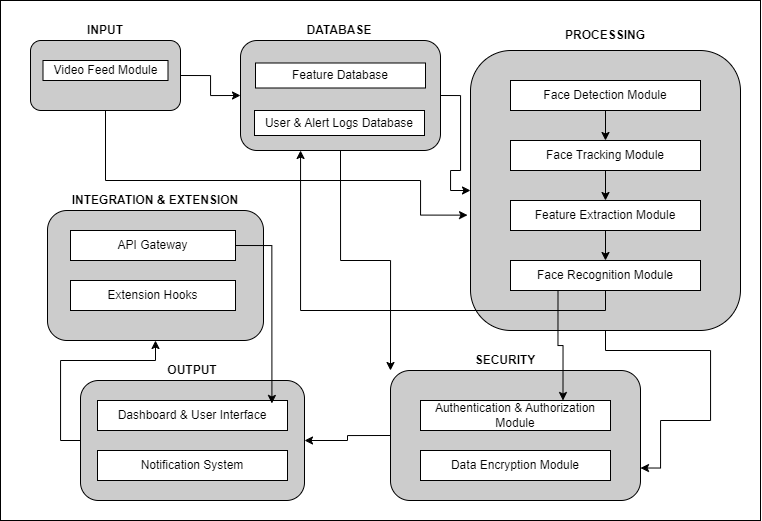
\includegraphics[width=0.75\textwidth]{components/images/sys-arch.png}
		\caption{System Architecture}
		\label{fig:sys-arch}
	\end{figure}

\section{UML Diagrams}
	\subsection{Use-case Diagram}
		\begin{figure}[h!]
			\centering
			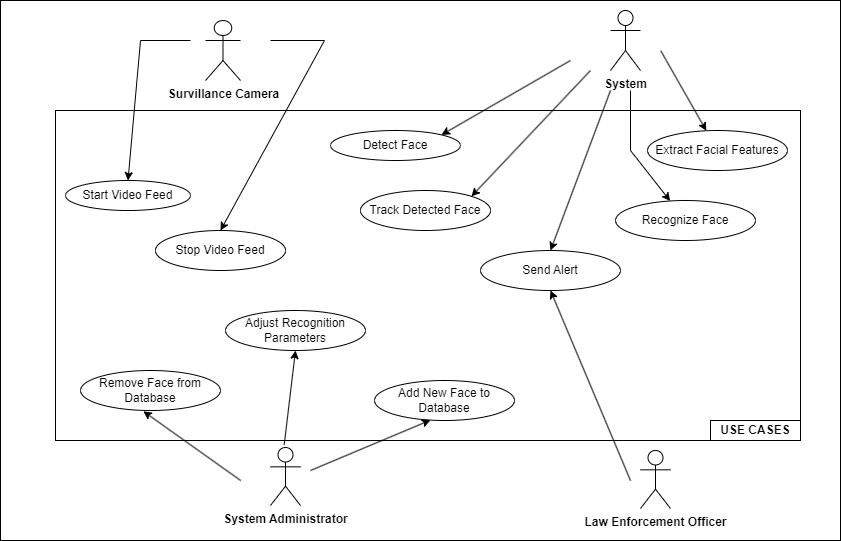
\includegraphics[width=0.75\textwidth]{components/images/use-case.png}
			\caption{Use-case Diagram}
			\label{fig:use-case-rep}
		\end{figure}

	\pagebreak

	\subsection{Sequence Diagram}
		\begin{figure}[h!]
			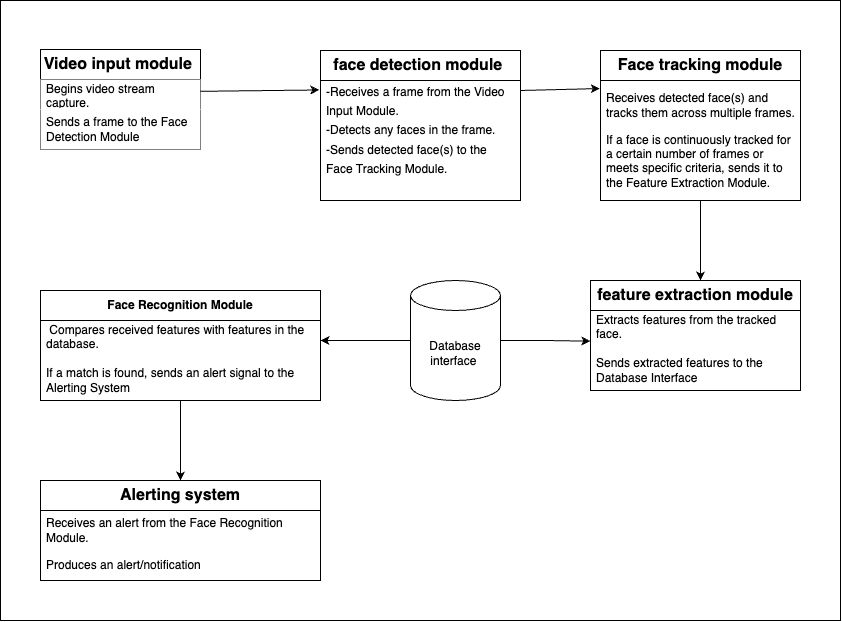
\includegraphics[width=\textwidth]{components/images/sequence.jpg}
			\caption{Sequence Diagram}
			\label{fig:sequence}
		\end{figure}

	\pagebreak

	\subsection{Activity Diagram}
		\begin{figure}[h!]
			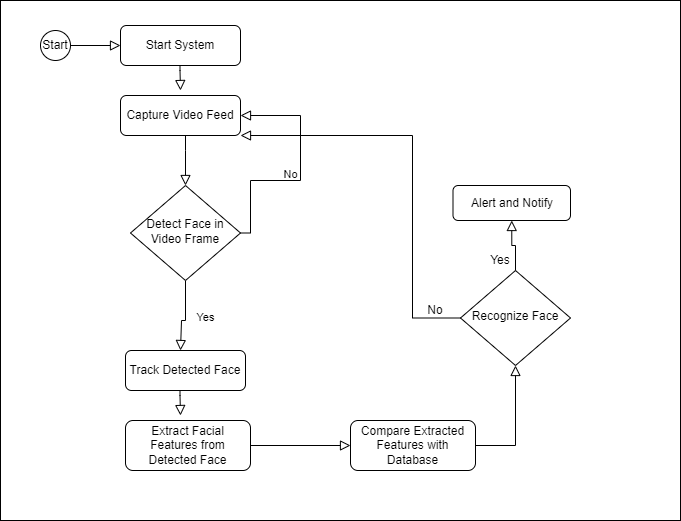
\includegraphics[width=\textwidth]{components/images/activity.png}
			\caption{Activity Diagram}
			\label{fig:activity}
		\end{figure}

	\pagebreak

	\subsection{State Diagram}
		\begin{figure}[h!]
			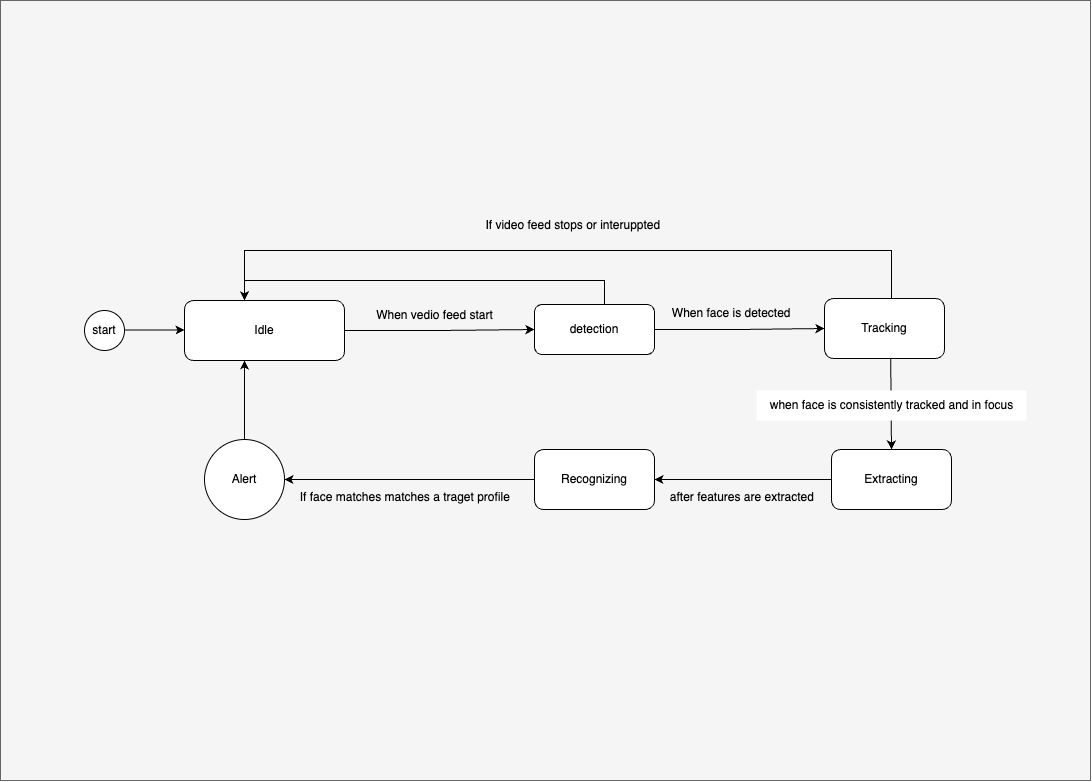
\includegraphics[width=\textwidth]{components/images/state.jpg}
			\caption{State Diagram}
			\label{fig:state}
		\end{figure}

	\pagebreak

	\subsection{Component Diagram}
		\begin{figure}[h!]
			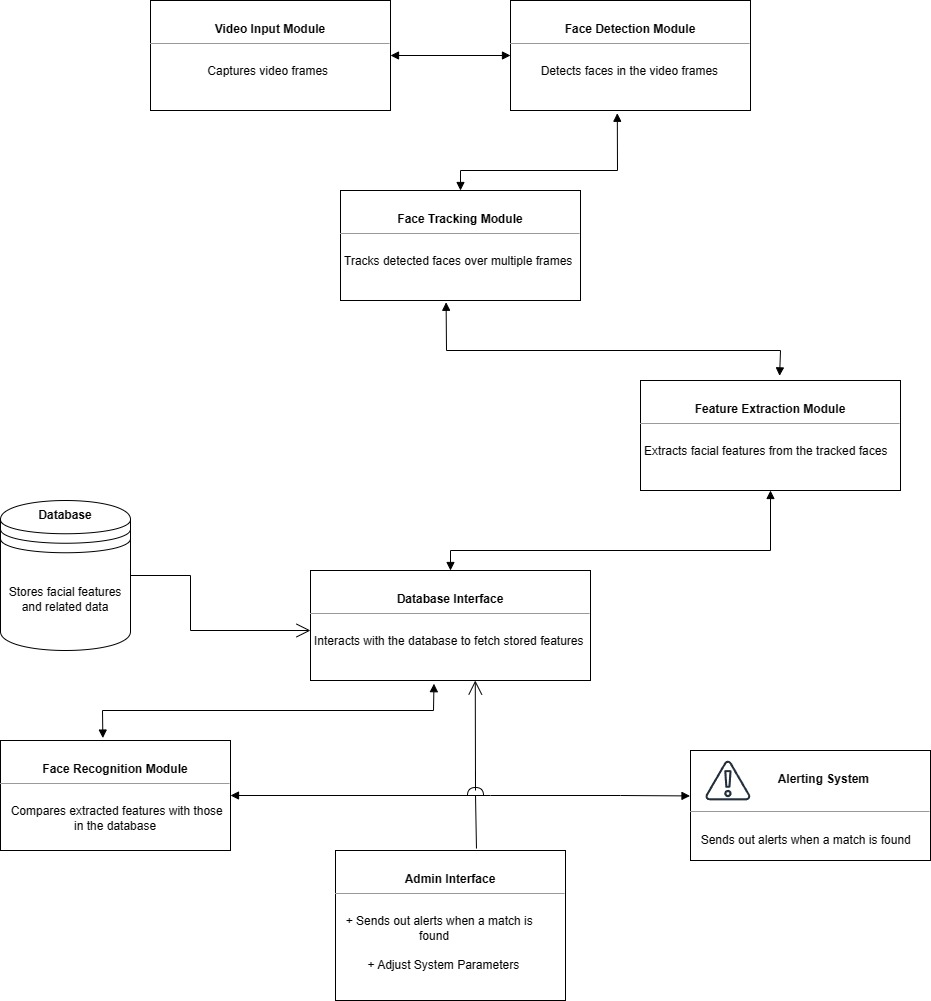
\includegraphics[width=\textwidth]{components/images/component.jpg}
			\caption{Component Diagram}
			\label{fig:component}
		\end{figure}

	\subsection{Class Diagram}
		\begin{figure}[h!]
			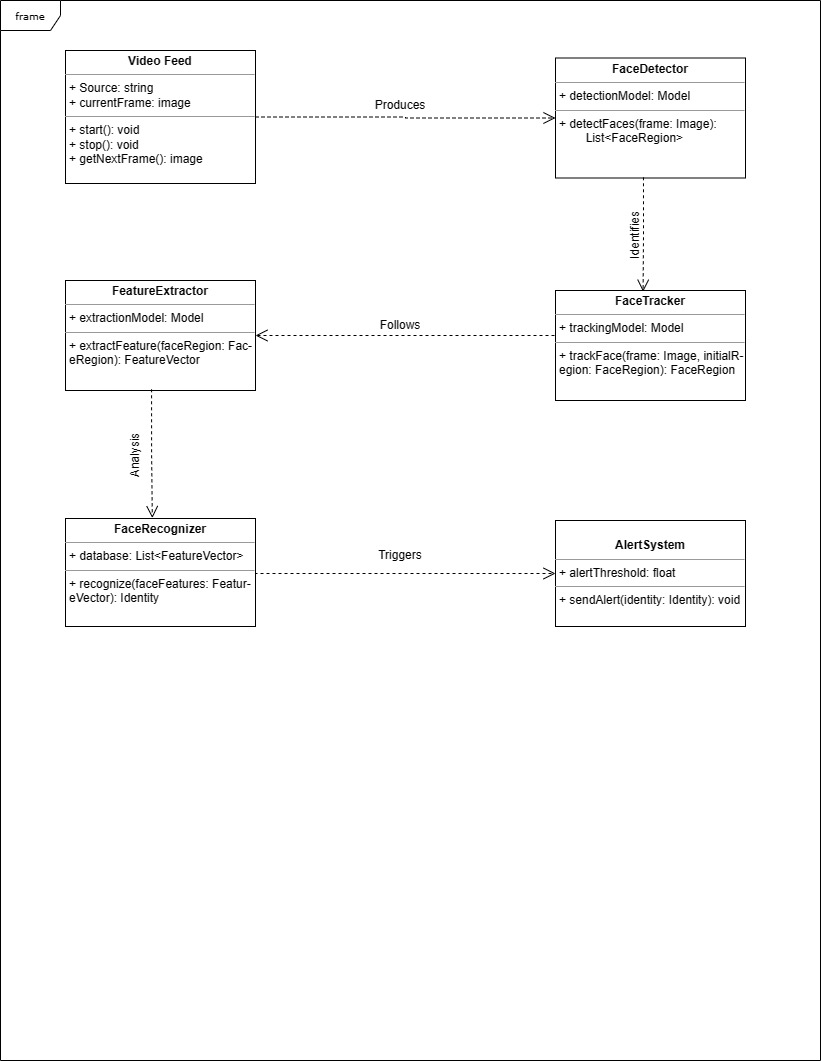
\includegraphics[width=\textwidth]{components/images/class.jpeg}
			\caption{Class Diagram}
			\label{fig:class}
		\end{figure}

	\pagebreak

	% \subsection{Object Diagram}
	% 	\begin{figure}[h!]
	% 		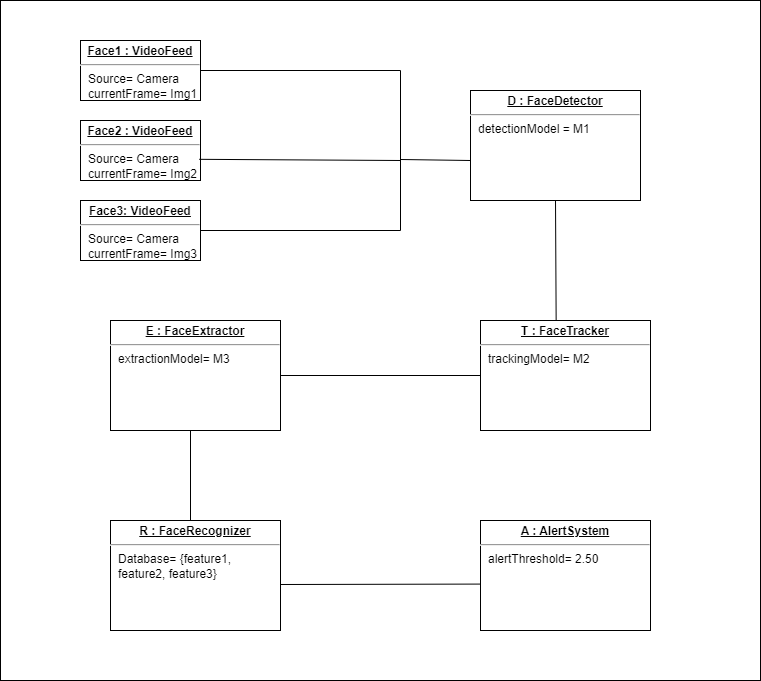
\includegraphics[width=\textwidth]{components/images/object.png}
	% 		\caption{Object Diagram}
	% 		\label{fig:object}
	% 	\end{figure}

	% \subsection{Deployment Diagram}
	% 	\begin{figure}[h!]
	% 		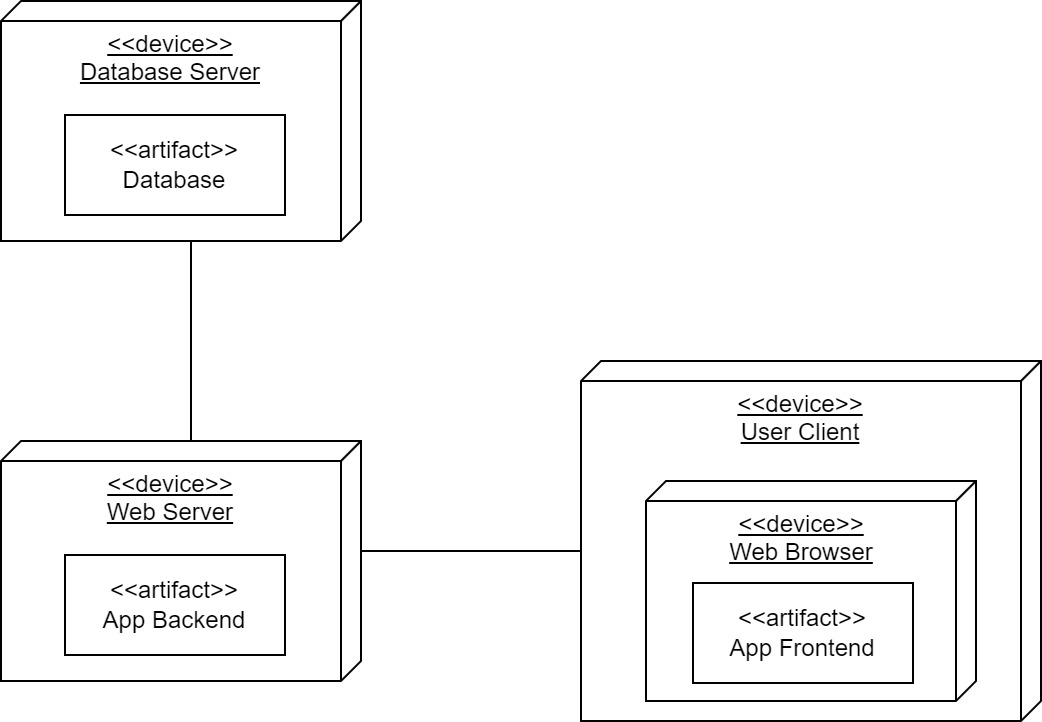
\includegraphics[width=\textwidth]{components/images/deployment.png}
	% 		\caption{Deployment Diagram}
	% 		\label{fig:deployment}
	% 	\end{figure}
	\chapter{Project Planning}

\section{Software Requirements}
	After literature survey and studies, the top tools that were found for our project are as follows:

	\begin{itemize}
		\item \textbf{Machine learning training:} PyTorch, LambdaCloud, Google Colab.
		\item \textbf{Machine learning inference:} ONNX Runtime.
		\item \textbf{Web backend:} Express.
		\item \textbf{Web frontend:} HTML, JS, CSS.
		\item \textbf{Database:} Faiss, Milvus, Annoy.
	\end{itemize}

\section{Hardware Requirements}
	In accordance to the software requirements, hardware requirements for our project are as follows:

	\begin{itemize}
		\item \textbf{User devices:} Smartphones, tablets, laptops, and desktop computers.
		\item \textbf{Cameras:} CCTVs.
		\item \textbf{CPU:} Multi-core 2.5 GHz.
		\item \textbf{GPU:} Minimum 8GB VRAM for training.
		\item \textbf{Internet connectivity:} Stable internet connection.
	\end{itemize}

\section{Project Timeline}
	Probable date of project completion is by the end of the term. A month-by-month distribution and estimation of milestones is as follows:

	\begin{table}[h!]
		\renewcommand{\arraystretch}{1.5}
		\caption{Project Timeline}
		\label{table:timeline}
		\begin{tabularx}{\columnwidth}{
			>{\centering\arraybackslash}p{1.5cm}
			X
		}
			\toprule
				\textbf{Month} & \textbf{Milestones} \\
			\midrule
				1 & Team formation, guide allocation, ideation and topic finalization. \\
				2 & Literature review, feasibility study, scope finalization. \\
				3 & Requirement analysis, high-level architecture design. \\
				4 & Stage-I review. \\
			\addlinespace \hline \addlinespace
				5 & Prototyping, data collection, pipeline setup. \\
				6 & Development and integration. \\
				7 & Testing, optimization, polish. \\
				8 & Stage-II review. \\
			\addlinespace \hline \addlinespace
				Future & Continuous integration and deployment. \\
			\bottomrule
		\end{tabularx}
	\end{table}
	\chapter{CONCLUSION}

In this preliminary project report, we discuss this project's core objective, which was to address the persistent challenges of real time face recognition in the wild for law enforcement scenarios. To this end, we designed a real time face recognition system which can detect faces in the wild in real time. The project is not only about enhancing user experiences but also about promoting enhanced public safety. By identifying individuals of interest in real-time, we tend to create a system in which law enforcement can act proactively to prevent crimes or apprehend suspects more efficiently. Swift and accurate identification of individuals can lead to timely interventions, preventing potential security threats and ensuring the safety of the public.


	\bibliographystyle{IEEEtranN.bst}
	\bibliography{
		components/refs/settings.bib,
		components/refs/all.bib
	}
\end{document}